\documentclass[twocolumn,a4paper,10pt]{my_report}

\title{Relazione sul laboratorio di metodologie biomolecolari}
\author{Margherita Martina Lo Campo}
\date{\today}

\begin{document}

\header{Laboratorio Metodologie Biomolecolari}{
Corso di Laurea Triennale in Scienze Biologiche \\
Anno Accademico 2017-2018 \\
Modulo: Biologia Molecolare -- Professor Solomon Nergadze}

\section{Esperimento 1 -- Reazione a catena della polimerasi (PCR) -- 6--03--2018}

\subsection{Scopo dell’esperimento}
L'obiettivo è quello di amplificare un frammento di DNA inserito in un vettore plasmidico.
Questa tecnica rientra nella categoria di metodi per il clonaggio, ossia permette di ottenere un numero elevato di copie di un frammento di DNA di interesse, che inseriamo in un vettore plasmidico.
Quest’ultimo consiste in una molecola di DNA a doppia elica, che si trova nel citoplasma delle cellule batteriche.
Il termine ``vettore'' indica il ruolo di trasportatore del plasmide, che contiene l'inserto.

La PCR sfrutta la funzione della DNA polimerasi, enzima che in presenza di nucleotidi, primer ed altre componenti, permette di amplificare un determinato frammento a partire da un templato, ossia uno stampo che nel caso di questo esperimento è proprio il vettore plasmidico.
Affinché ciò avvenga è necessario che si conoscano le estremità del frammento che si vuole amplificare al fine di creare i primer forward e reverse (rispettivamente complementari ai filamenti $3' \rightarrow 5'$ e $5' \rightarrow 3'$) che andranno ad appaiarsi al templato e faranno da innesco alla DNA Polimerasi.
In provetta, si inseriscono i primer, i nucleotidi (dNTPs) che sono utilizzati dalla polimerasi per formare il nuovo filamento, il Buffer colorless ossia un tampone incolore che crea le condizioni ideali per la polimerasi, il magnesio che costituisce un importate coenzima che coadiuva l’attività enzimatica della polimerasi, la Taq polimerasi ossia una DNA polimerasi termoresistente isolata nel batterio Thermus acquaticus.

\begin{figure}[htbp]
\centering
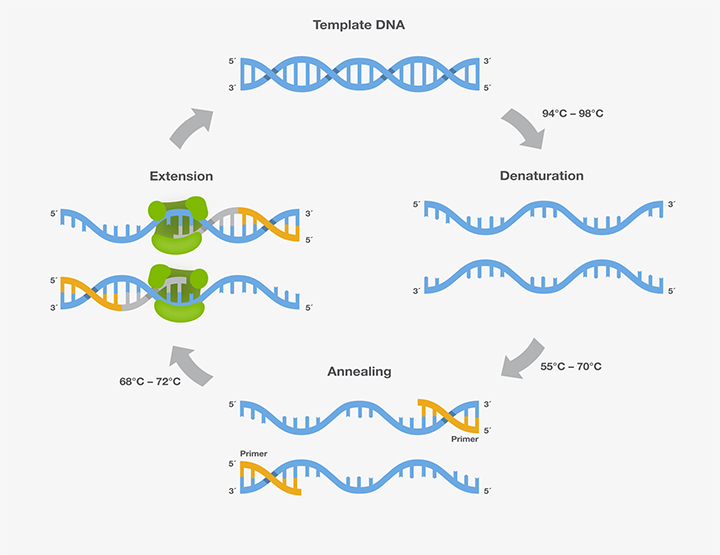
\includegraphics[width=0.8\linewidth]{1.jpg}
\caption{Schema grafico fasi PCR}
\label{fig:FasiPCR}
\end{figure}

La PCR si compone di più fasi; la \emph{denaturazione} prevede l’esposizione del DNA ad alte temperature (circa \SI{90}{\celsius}) che porta alla rottura dei ponti idrogeno presenti tra le basi azotate in modo da separare i filamenti e renderli liberi in provetta, assieme agli altri reagenti.
A seguire abbiamo la fare di \emph{annealing}, durante la quale i primer prima citati, presenti in provetta, vanno ad appaiarsi ai filamenti di DNA determinando le estremità del frammento da amplificare; nota importante di questa fase è l’abbassamento della temperatura a circa \SIrange{56}{63}{\celsius} per poter permettere il legame primer--DNA.
Nella successiva terza ed ultima fase, \emph{allungamento}, la temperatura viene rialzata sino ai \SIrange{75}{80}{\celsius} che risulta essere la temperatura ottimale per la Taq Polimerasi. Queste tre fasi, si ripetono per un totali di circa 35 cicli in un macchinario noto come termociclatore, in modo da ottenere il nostro inserto di DNA amplificato.

\subsection{Protocollo}
Tramite utilizzo di pipette automatiche Gilson (p20-p200-p1000), si preparano due provette Eppendorf, contenenti due soluzioni così composte:
\begin{itemize}
	\item provetta 1 ``Mix'':
	\begin{itemize}
	    \item \SI{3}{\ul} di Primer Mix (contenente sia il reverse che il foreword)
    	\item \SI{10}{\ul} di dNTPs (\SI{1}{\milli\Molar})
    	\item \SI{10}{\ul} di Buffer colorless
    	\item \SI{6}{\ul} di \ch{MgCl2}(\SI{25}{\milli\Molar})
    	\item \SI{0.5}{\ul} di Taq polimerasi
    	\item \SI{20.5}{\ul} di \ch{H2O}. Questa provetta conterrà la soluzione di controllo, al fine di verificare che il lavoro svolto nella provetta 2 sia corretto.
	\end{itemize}
	\item provetta 2 ``PCR'':
	\begin{itemize}
		\item \SI{3}{\ul} di Primer Mix (\SI{10}{\micro\Molar} contenente sia il reverse che il foreword)
    	\item \SI{10}{\ul} di dNTPs (\SI{1}{\milli\Molar})
    	\item \SI{10}{\ul} di Buffer colorless
    	\item \SI{6}{\ul} di \ch{MgCl2} (\SI{25}{\milli\Molar})
    	\item \SI{0.5}{\ul} di Taq polimerasi
    	\item \SI{15.5}{\ul} di \ch{H2O}
    	\item \SI{5}{\ul} di DNA plasmidico (\SI{1}{\micro\Molar}).
	\end{itemize}
\end{itemize}
In entrambe le provette si avrà un totale di \SI{50}{\ul} di soluzione; queste verranno messe nel termociclatore e una volta terminati i cicli di amplificazione, si otterranno $2^{n-2}$ frammenti (dove l'esponente indica il numero dei cicli meno i frammenti persi).
Si prelevano \SI{10}{\ul} dalla provetta 2 PCR e si mescolano con \SI{2}{\ul} di loading dye, ossia un buffer colorato il cui volume lo si ricava applicando la formula $V_i \cdot C_i = V_f \cdot C_f$, facendo poi un ``quick run'' ossia una mescolatura tramite breve centrifugazione.
Lo stesso procedimento va fatto con la provetta1 Mix. Questi \SI{12}{\ul} risultanti si caricano su gel di agarosio, per l’elettroforesi.

Il gel di agarosio è composto da:
\begin{itemize}
    \item TAE (Tris acetato ed EDTA), ossia un buffer concentrato al 40\%. Nel nostro caso per \SI{300}{\ml} di soluzione andremo a calcolarci il volume necessario di TAE con la formula $V_i \cdot C_i = V_f \cdot C_f$ affinchè si ottenga una soluzione concentrata all’1\% di TAE.
    \item Agarosio: \SI{1}{\gram} per ogni \SI{100}{\ml} di soluzione, nel nostro caso si aggiungeranno \SI{3}{\gram} di agarosio nella soluzione.
    \item \ch{H2O}
    \item Etidio bromuro: un colorante che interagisce con il DNA e una volta irraggiato da UV emette fluorescenza. Si aggiungono \SI{5}{\ul} di colorante per ogni \SI{100}{\ml} di soluzione, per un totale di \SI{15}{\ul}.
\end{itemize}
N.B. in laboratorio si usa il Real Safe, una sostanza meno tossica dell’etidio bromuro.

Il gel viene messo in vasca assieme al pettine che formerà i pozzetti una volta solidificato il gel; successivamente viene fornita una differenza di potenziale alla vasca elettroforetica che permette al DNA caricato nei pozzetti di migrare verso il polo positivo, poiché dotato di carica negativa per via dei gruppi fosfato.
I frammenti più piccoli tenderanno a correre più velocemente sul gel, mentre quelli con un peso molecolare maggiore tenderanno a correre più lentamente attraverso le maglie del gel, infatti la velocità del frammento è inversamente proporzionale al logaritmo della lunghezza.

\subsection{Risultati ed interpretazione}
Il risultato dopo analisi elettroforetica è visibile in \hl{fig.}~\ref{fig:pcr}.
Sono visibili tre colonne: nella prima possiamo notare le bande relative al marcatore scala 1Kb dove ciascuna banda rappresenta un frammento di DNA di dimensioni diverse; nella seconda colonna (+) notiamo un'unica banda, la cui dimensione è circa 600pb, corrispondente al frammento che si voleva amplificare; nella terza colonna (-), notiamo una banda meno marcata, posta più in basso rispetto alla banda dell’amplificato.
Quest’ultima infatti corrisponde alla nostra provetta 1 Mix nella quale non era presente DNA; il buffer infatti corre più velocemente su gel di agarosio motivo per il quale la banda è posta più giù rispetto a quella del nostro amplificato.
Non avendo notato nessuna amplificazione in corrispondenza della Mix possiamo dedurre che il lavoro è stato svolto correttamente e senza alcuna contaminazione.

\section{Esperimento 2 -- Digestione con enzimi di restrizione e costruzione di una mappa di restrizione -- 7--03--2018/8--03--2018}

\subsection{Scopo dell' esperimeto}
In questo esperimento si ha il plasmide pGEM, un vettore per il clonaggio di geni in E.coli che porta come marcatore selettivo il gene che conferisce la resistenza all’antibiotico ampicillina (amp).
È inoltre presente un’origine di duplicazione (ori) che permette al plasmide di replicarsi nelle cellule batteriche.
Le cellule che contengono il plasmide si distinguono da quelle che ne sono prive poiché vengono coltivante in un terreno contenente l’amp.
In questo vettore è stato inserito un frammento di DNA genomico di Gibbone, il cui taglio è stato operato da un enzima di restrizione noto come EcoRI.
Nel corso dell’esperimento verranno operate delle digestioni di diversi tipi di DNA (plasmide pGEM-ins, DNA genomico di E.coli e DNA genomico umano) con diversi enzimi di restrizione.
I frammenti ottenuti da queste digestioni verranno separati tramite elettroforesi su gel di agarosio in modo da determinarne i pesi molecolari.
La mappa di restrizione del plasmide verrà dedotta dall’analisi dei frammenti di restrizione.
Gli enzimi di restrizione sono endonucleasi che riconoscono determinate sequenze e in corrispondenza di queste operano un taglio; quelle da noi adoperate sono:
\begin{itemize}
	\item EcoRI: opera un taglio in corrispondenza della sequenza
	\begin{center}
    \begin{tikzpicture}[thick,>=latex]
    \sffamily\footnotesize
    \foreach \x[count=\xi] in {5',\ldots,G,A,A,T,T,C,\ldots,3'}{\node[inner sep=0] (u-\xi) at (0.35*\xi,0.5){\x};}
    \foreach \x[count=\xi] in {3',\ldots,C,T,T,A,A,G,\ldots,5'}{\node[inner sep=0] (d-\xi) at (0.35*\xi,0){\x};}
    \draw [densely dashed, red, >-<] ($(1.05,1)!0.5!(1.4,1)$)|-($(u-6)!0.5!(d-6)$)-|($(2.45,-0.5)!0.5!(2.8,-0.5)$);
    \end{tikzpicture}
	\end{center}
	\item ScaI: opera un taglio in corrispondenza della sequenza
	\begin{center}
    \begin{tikzpicture}[thick,>=latex]
    \sffamily\small\footnotesize
    \foreach \x[count=\xi] in {5',\ldots,A,G,T,A,C,T,\ldots,3'}{\node[inner sep=0] (u-\xi) at (0.35*\xi,0.5){\x};}
    \foreach \x[count=\xi] in {3',\ldots,T,C,A,T,G,A,\ldots,5'}{\node[inner sep=0] (d-\xi) at (0.35*\xi,0){\x};}
    \draw [densely dashed,red, >-<] ($(1.75,1)!0.5!(2.1,1)$)--($(1.75,-0.5)!0.5!(2.1,-0.5)$);
    \end{tikzpicture}
	\end{center}
	\item HinfI: opera un taglio in corrispondenza della sequenza
	\begin{center}
    \begin{tikzpicture}[thick,>=latex]
    \sffamily\small\footnotesize
    \foreach \x[count=\xi] in {5',\ldots,G,A,N,T,C,\ldots,3'}{\node[inner sep=0] (u-\xi) at (0.35*\xi,0.5){\x};}
    \foreach \x[count=\xi] in {3',\ldots,C,T,N,A,G,\ldots,5'}{\node[inner sep=0] (d-\xi) at (0.35*\xi,0){\x};}
    \draw [densely dashed, red, >-<] ($(1.05,1)!0.5!(1.4,1)$)|-($(u-5)!0.5!(d-5)$)-|($(2.1,-0.5)!0.5!(2.45,-0.5)$);
    \end{tikzpicture}
	\end{center}
\end{itemize}

Ciascuno di questi enzimi ha un proprio sito di restrizione, presente una sola volta nel polycloning site contenuto nel vettore plasmidico.
Un vettore ideale deve essere capace di replicarsi autonomamente, deve contenere un marcatore che lo renda distinguibile e deve essere facile da isolare dalle cellule ospite.
Dopo aver operato con questi enzimi si otterranno $(\sfrac{1}{4})^{n}$ frammenti di restrizione\footnote{Dove $n$ ci indica il numero di basi riconosciute per il taglio.}.

\subsection{Protocollo}
\begin{table*}[htbp]
\sffamily\scriptsize
\centering
%\setlength\extrarowheight{3pt}
\input{table1.tab}
\caption{\label{tab:dna} Vengono usati i tamponi E--S e H rispettivamente per le soluzioni contenenti EcoRI/ScaI e per quelle contenenti HinfI, al fine di creare le condizioni ideali per ciascun enzima di restrizione. I campioni (1--5--8) non sono trattati con enzimi di restrizione, mentre il campione 4 è sottoposto ad una doppia digestione enzimatica; questo viene fatto per aver modo di comparare i campioni con singola o doppia digestione ai campioni nei quali non viene operato nessun taglio endonucleasico.}
\end{table*}

Si allestiscono dodici provette Eppendorf, numerate, contenenti ciascuna un volume totale di soluzione pari a \SI{20}{\ul} come riportato in tabella~\ref{tab:dna}.
Una volta ultimata la preparazione delle dodici Eppendorf, si mettono i campioni in incubatrice a \SI{37}{\celsius} per circa un’ora.
Al termine di questa operazione, prima di caricare i campioni ormai digeriti su gel di agarosio per la corsa elettroforetica, si aggiunge a ciascuna Eppendorf il loading dye (6X).
Una volta prelevati e aggiunti con una pipetta Gilson p20, \SI{4}{\ul} di loading dye alle soluzioni, si fa una quick run per assicurare un buon mescolamento.
Il loading dye è composto da glicerolo, un componente necessario affinché il campione si appesantisca e si depositi bene sul fondo del pozzetto, da colorante (blu di bromo fenolo) che permette di tracciare la corsa dei frammenti di DNA durate elettroforesi.

Terminata questa fase, si caricano le dodici soluzioni su gel di agarosio concentrato 0.8\%, preparato con gli stessi reagenti visti e descritti nella prima giornata di laboratorio; tuttavia la concentrazione è relativamente più bassa poiché si devono separare frammenti con una lunghezza maggiore.
Il principio alla base di ciò è che il gel di agarosio forma una trama a maglie tanto più serrate quanto più è concentrato, dunque un gel più concentrato avrà un’efficacia maggiore per la separazione di frammenti di DNA più piccoli.
Al termine della corsa elettoforetica, la foto del gel assieme all’impiego dei marcatori λ--Hind e Scala 250pb permettono di costruire due curve di taratura \hl{come visibile in fig.}~\ref{fig:scaI} \hl{e fig.}~\ref{fig:hind} e di risalire alle dimensioni dei frammenti con un peso molecolare non noto.
Per ottenere la prima curva si misura la distanza (\si{mm}) che intercorre tra l’inizio della corsa e ciascuno dei frammenti HindIII del marcatore λ--Hind; per la seconda curva si procede allo stesso modo tenendo però in considerazione il marcatore Scala 250pb il quale indica una distanza di 250pb tra una banda e l’altra.

\subsection{Risultati ed interpretazione}
Dalla foto del gel dopo elettroforesi (\hl{vedi fig.}~\ref{fig:pcr2}), possiamo vedere chiaramente dodici bande, dieci delle quali rappresentano le nostre soluzioni contenenti DNA diversi, digeriti con gli enzimi di restrizione prima citati, le ultime due rappresentano i nostri marcatori λ-Hind e Scala 250pb.

Come premessa per una buona comprensione dei risultati è importante tener presente che una banda corrisponde ad un frammento di DNA prodotto dalla digestione e che dunque consiste in un insieme di molecole di DNA della stessa lunghezza che corrono con la stessa velocità.
Inoltre un plasmide ha configurazioni diverse; se il plasmide è superavvolto risulterà essere più piccolo, strettamente impacchettato e dunque più veloce nella corsa elettrofertica, tuttavia sarà impossibile dedurne il peso molecolare fino a quando questo non verrà linearizzato tramite taglio endonucleasico con enzimi di restrizione.

\hl{In fig.}~\ref{fig:pcr2} notiamo che nella prima colonna (pGEM-ins non digerito) abbiamo due bande: una più marcata e posta più in alto che rappresenta il plasmide sotto forma di aggregato di molecole, un’altra posta più in basso e leggermente più chiara che rappresenta il plasmide superavvolto e dunque più veloce.
Nella seconda colonna (pGEM-ins digerito con EcoRI) abbiamo due bande, una molto più marcata con un peso molecolare di circa 3000pb e l’altra meno evidente con un peso molecolare di circa 600pb.
Nella terza colonna (pGEM-ins digerito con ScaI) abbiamo un unico frammento con un peso molecolare di circa 3600pb.
In quarta colonna (pGEM-ins con doppia digestione EcoRI-ScaI) osserviamo 3 bande di cui una con un peso molecolare di circa 1800pb, una banda posta più in basso di circa 1250pb e l’ultima ancora più piccola di 600pb analoga alla banda notata nella terza colonna.

Con questi dati concludiamo che il plasmide pGEM-ins viene dapprima tagliato con EcoRI il quale in corrispondenza del proprio sito di taglio, crea due frammenti, uno piccolo (600pb) e l’altro grande (3000pb).
Poi abbiamo la digestione del plasmide con ScaI, il quale pratica un unico taglio linearizzando il plasmide, creando una banda di 3600pb.
In seguito a doppia digestione invece abbiamo dapprima EcoRI la cui azione crea due frammenti, poi ScaI interviene sul frammento più grande per ottenere un totale di tre frammenti.
Il frammento più piccolo (600pb) è il nostro inserto e la somma dei pesi molecolari dei tre frammenti generati dalla doppia digestione ci fornisce il peso moleclare del pGEM-ins (\hl{vedi fig.}~\ref{fig:pGEM}).

\begin{figure}[htbp]
\centering
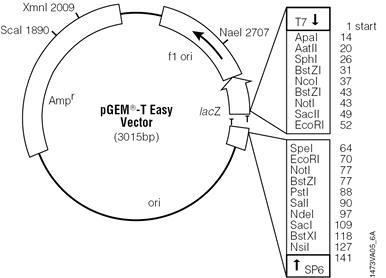
\includegraphics[width=0.8\linewidth]{2.jpg}
\caption{Mappa di restrizione pGEM}
\label{fig:pGEM}
\end{figure}

Un caso particolare si nota invece in colonna sei (DNA umano digerito con EcoRI) e sette (DNA umano digerito con HinfI); quello che otteniamo dalla corsa elettroforetica è rispettivamente uno smear concentrato verso l’alto e uno smear concentrato verso il basso; questo perché EcoRI (un six cutter) produce frammenti più grandi di HinfI (un four cutter).
Uno smear è una striscia non nitida, nella quale non sono riconoscibili bande.
EcoRI usato in colonna sei produce $(\sfrac{1}{4})^6$ frammenti, di lunghezza più grande rispetto a HinfI che produce $(\sfrac{1}{4})^4$ frammenti di lunghezza minore; si ottengono dunque frammenti con lunghezze tanto simili da non evidenziare differenze nette tra una banda e l’altra.
Ciò è dovuto sia alla maggior grandezza del genoma umano, sia al fatto che EcoRI e HinfI hanno più siti di taglio in questo caso.

\section{Esperimento 3 -- Estrazione di DNA genomico da E. Coli -- 9--03--2018}

\subsection{Scopo dell’esperimento}
In questo esperimento ogni studente deve allestire una coltura di E.coli in terreno liquido LB, a partire da una singola colonia su piastra. Lo scopo sarà quello di eliminare la parete cellulare batterica, gli altri elementi subcellulari e ottenere in provetta solo il DNA batterico.

\subsection{Protocollo}
All’inizio dell’esperimento viene presentata una coltura di E.coli in terreno liquido, contenuta in una beuta, preparata dal Prof. Nergadze, che è stata fatta crescere per una notte a \SI{37}{\celsius} in bagno termostatato, contemporaneamente alle colture presenti in provetta che verranno utilizzate da noi. La beuta, essendo un contenitore più areato, permette una cresciuta migliore delle cellule batteriche, rispetto a quelle presenti in provetta. Per questo, \SI{2}{\ml} di coltura in beuta vengono aggiunti a \SI{8}{\ml} di coltura in provetta per un totale di \SI{10}{\ml} di terreno liquido LB.
La coltura presente in provetta, dopo aver ultimato la crescita, apparirà torbida per la presenza di un’elevata concentrazione di E.coli. L’estrazione del DNA viene fatta con i seguenti passaggi:

\begin{enumerate}
    \item centrifugare la coltura a 4000rpm per 8 minuti
    \item eliminare il supernatante (fase liquida in provetta) e lavare il pellet (fase contenente le cellule batteriche), risospendendolo in \SI{8}{\ml} di tampone TEN
    \item centrifugare la coltura a 4000rpm per 8 minuti
    \item eliminare il supernatante e riso spendere il pellet in \SI{1.350}{\ml} di tampone TEN--TX
    \item aggiungere \SI{150}{\ul} di una soluzione di lisozima (\SI{5}{\mg\per\ml})
    \item capovolgere alcune volte la provetta e incubare per 30 minuti a \SI{37}{\celsius}
    \item aggiungere \SI{0.1}{\mg\per\ml} di una soluzione di proteinasi K (\SI{10}{\mg\per\ml})
    \item incubare a \SI{65}{\celsius} per 30 minuti
    \item precipitare gli acidi nucleici aggiungendo due volumi di etanolo (circa \SI{4}{\ml}) concentrato al 96\% e capovolgere delicatamente diverse volte la provetta fino alla formazione di un gomitolo costituito prevalentemente da DNA batterico.
\end{enumerate}

Il tampone TEN è diverso dal tampone TEN--TX poiché quest’ultimo contiene detergente Triton X--100.
L’aggiunta di lisozima è necessaria affinchè la parete cellulare dei batteri venga distrutta; la proteinasi K invece digerisce la maggior parte delle cellule presenti nella cellula batteriche.
L’etanolo, sottrae molecole d’acqua causando la formazione di interazioni tra catene di una stessa molecola di DNA, così facendo si ottiene il ``gomitolo''.

\section{Risultati ed interpretazioni}
Il risultato di questo esperimento è stato il più formativo, a parer mio, poiché rende visibile concretamente ciò che studio da anni solo attraverso le pagine dei libri.
Avere il DNA in provetta è sicuramente una delle cose più stimolanti fatta in laboratorio.

\begin{figure}[htbp]
\begin{subfigure}{0.5\linewidth}
\centering
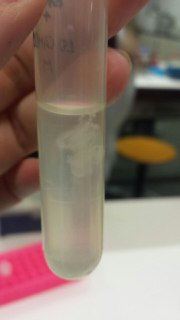
\includegraphics[width=0.8\linewidth]{3.jpg}
\label{fig:DNAunipv_a}
\end{subfigure}%
\begin{subfigure}{0.5\linewidth}
\centering
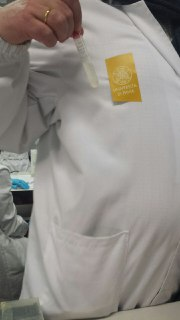
\includegraphics[width=0.8\linewidth]{4.jpg}
\label{fig:DNAunipv_b}
\end{subfigure}
\caption{Risultato della mia estrazione di DNA}
\label{fig:DNAunipv}
\end{figure}

\newpage
\onecolumn{
\section{Allegati modulo biologia molecolare}\label{sec:allegati_modulo1}
\begin{figure}[htbp]
\centering
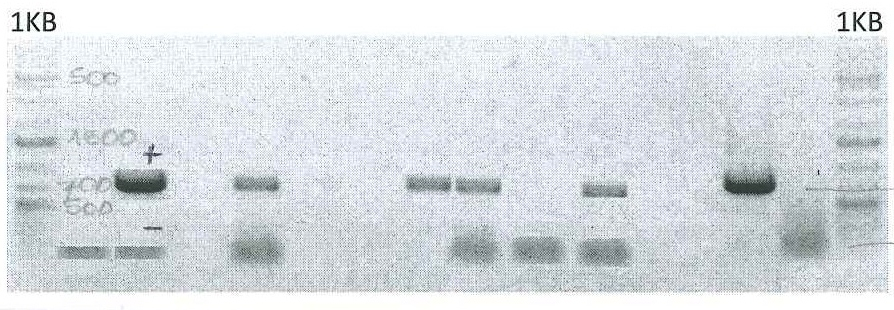
\includegraphics[width=0.8\linewidth]{pcr.jpg}
\caption{}
\label{fig:pcr}
\end{figure}

\begin{figure}[htbp]
\centering
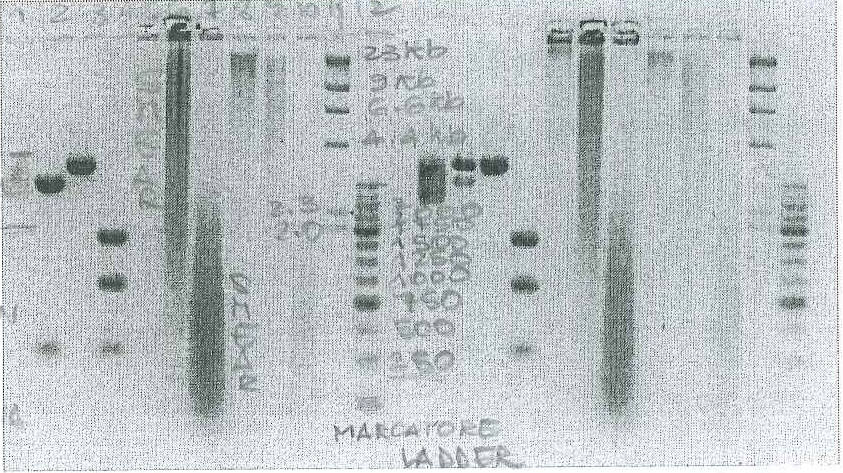
\includegraphics[width=0.8\linewidth]{pcr2.jpg}
\caption{}
\label{fig:pcr2}
\end{figure}

\begin{figure}
\centering
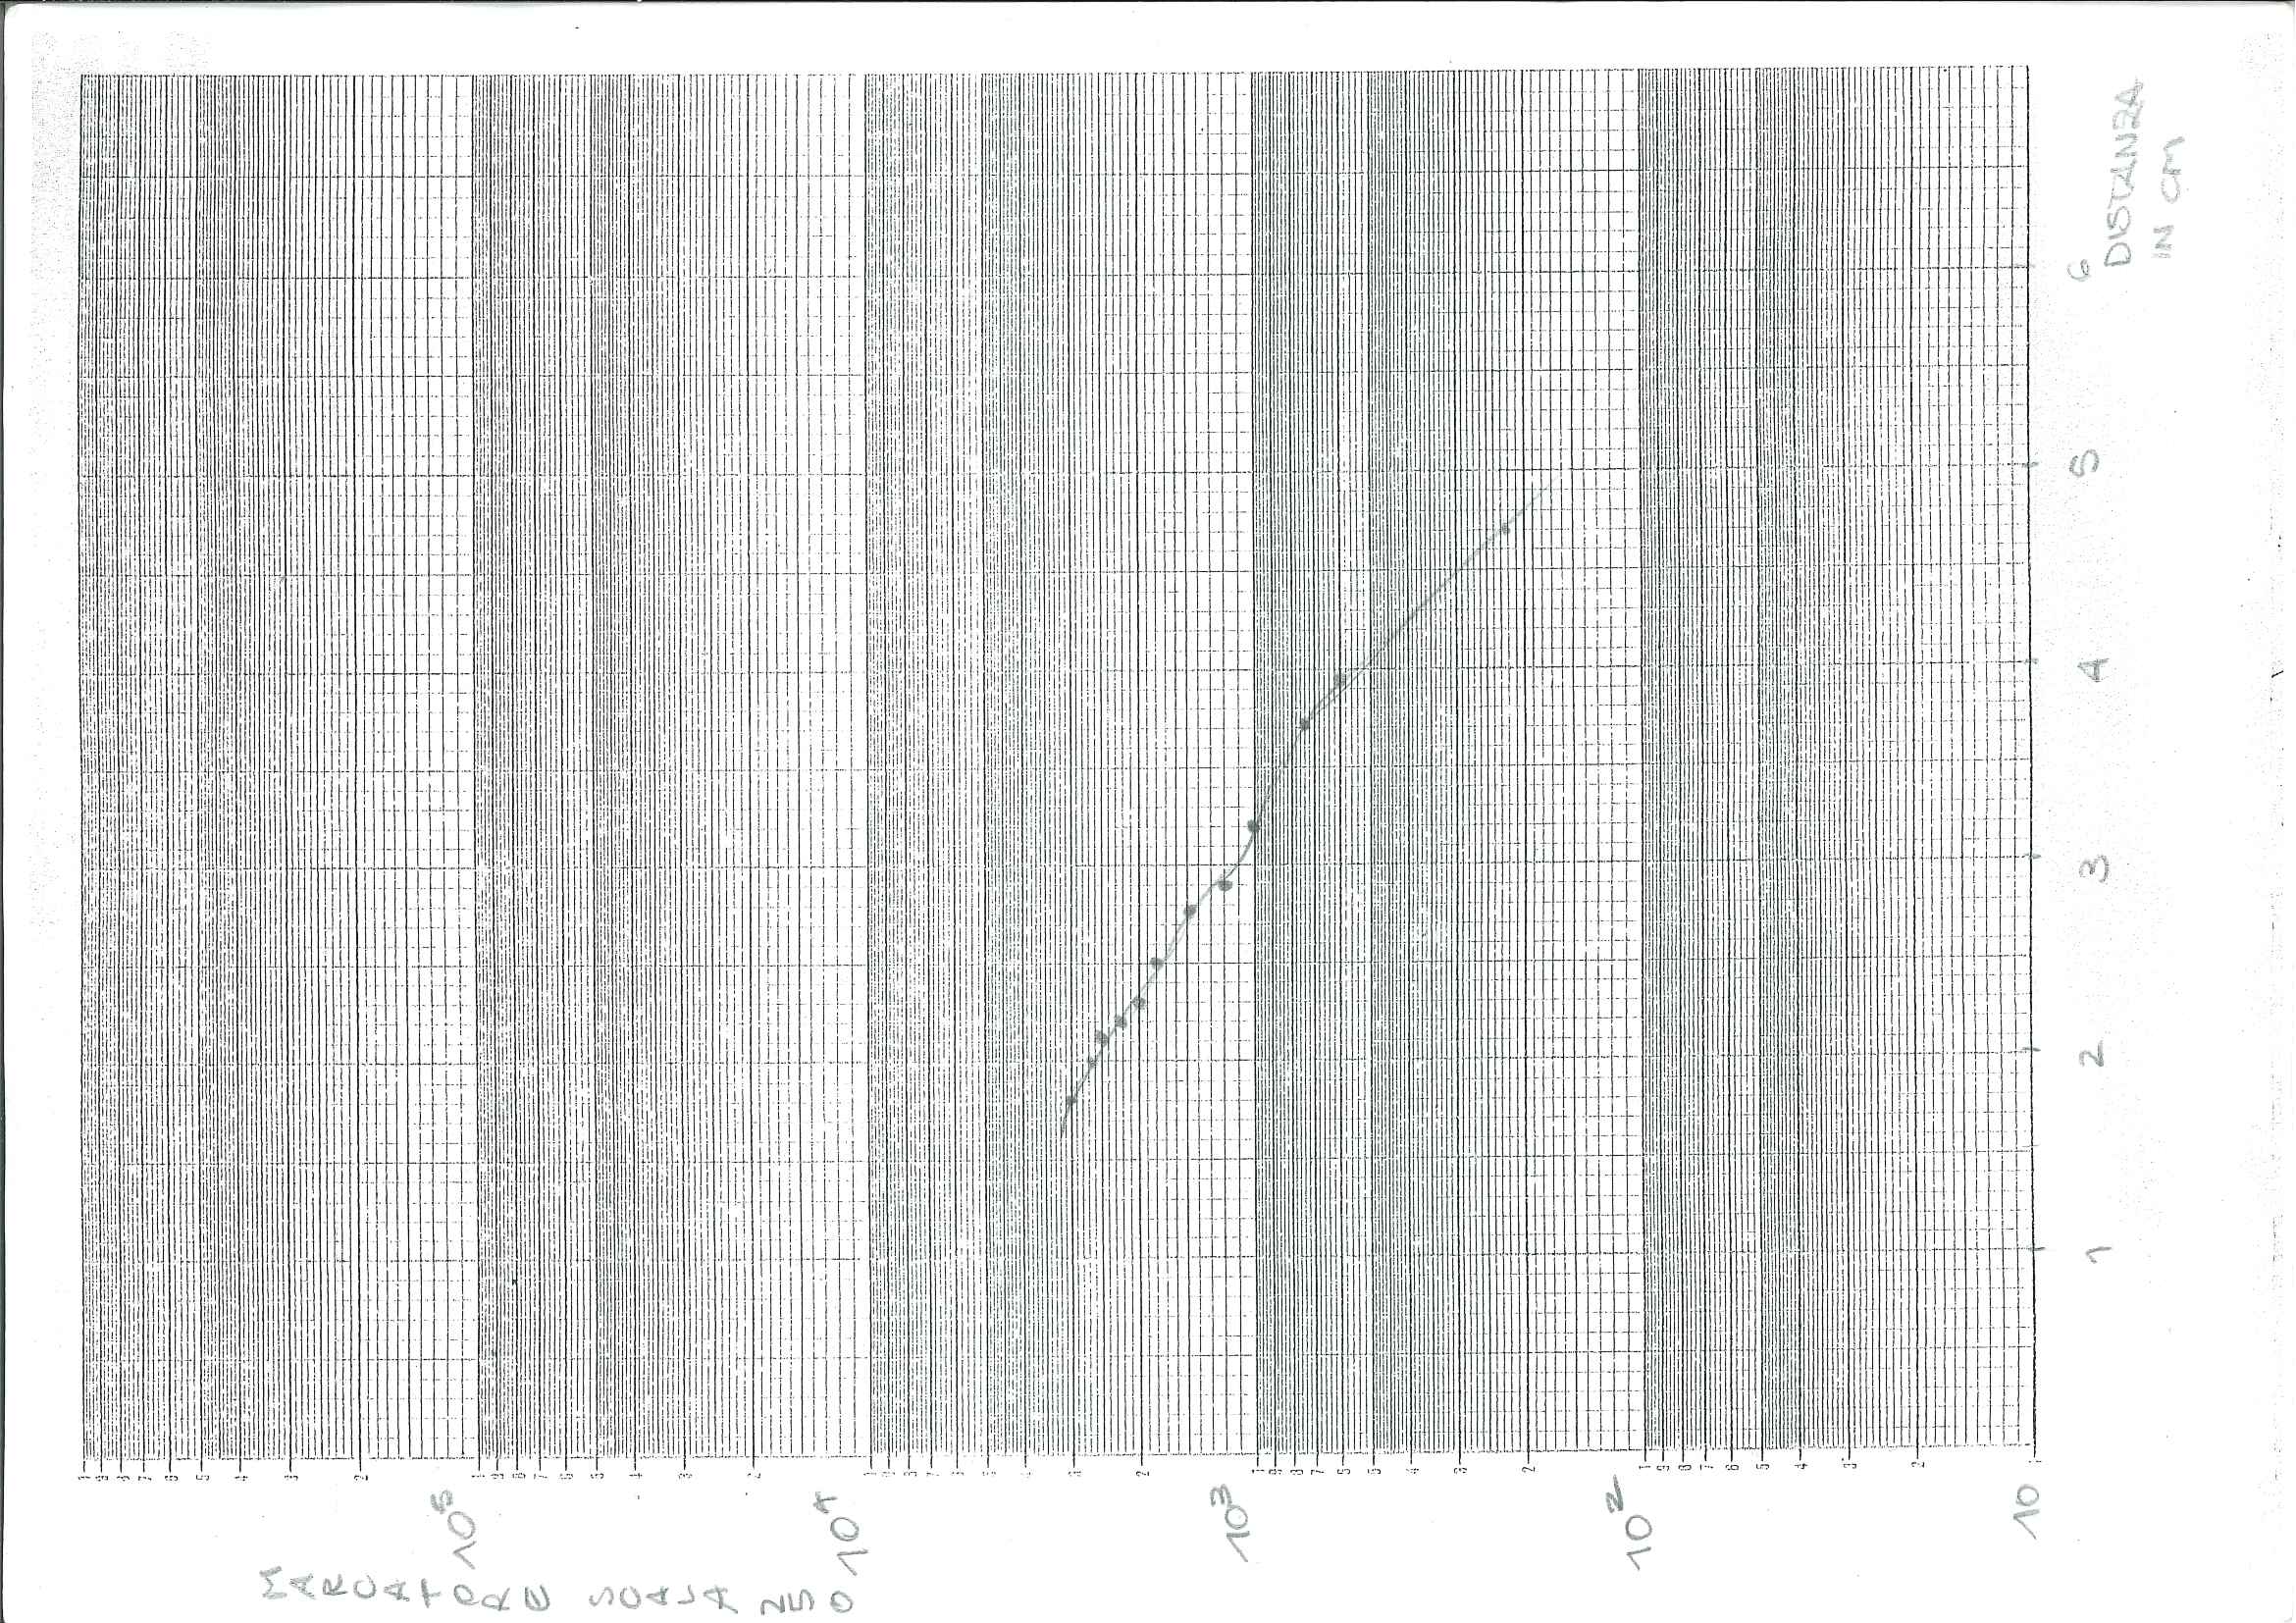
\includegraphics[width=0.8\linewidth]{scaI.jpg}
\caption{}
\label{fig:scaI}
\end{figure}

\begin{figure}
\centering
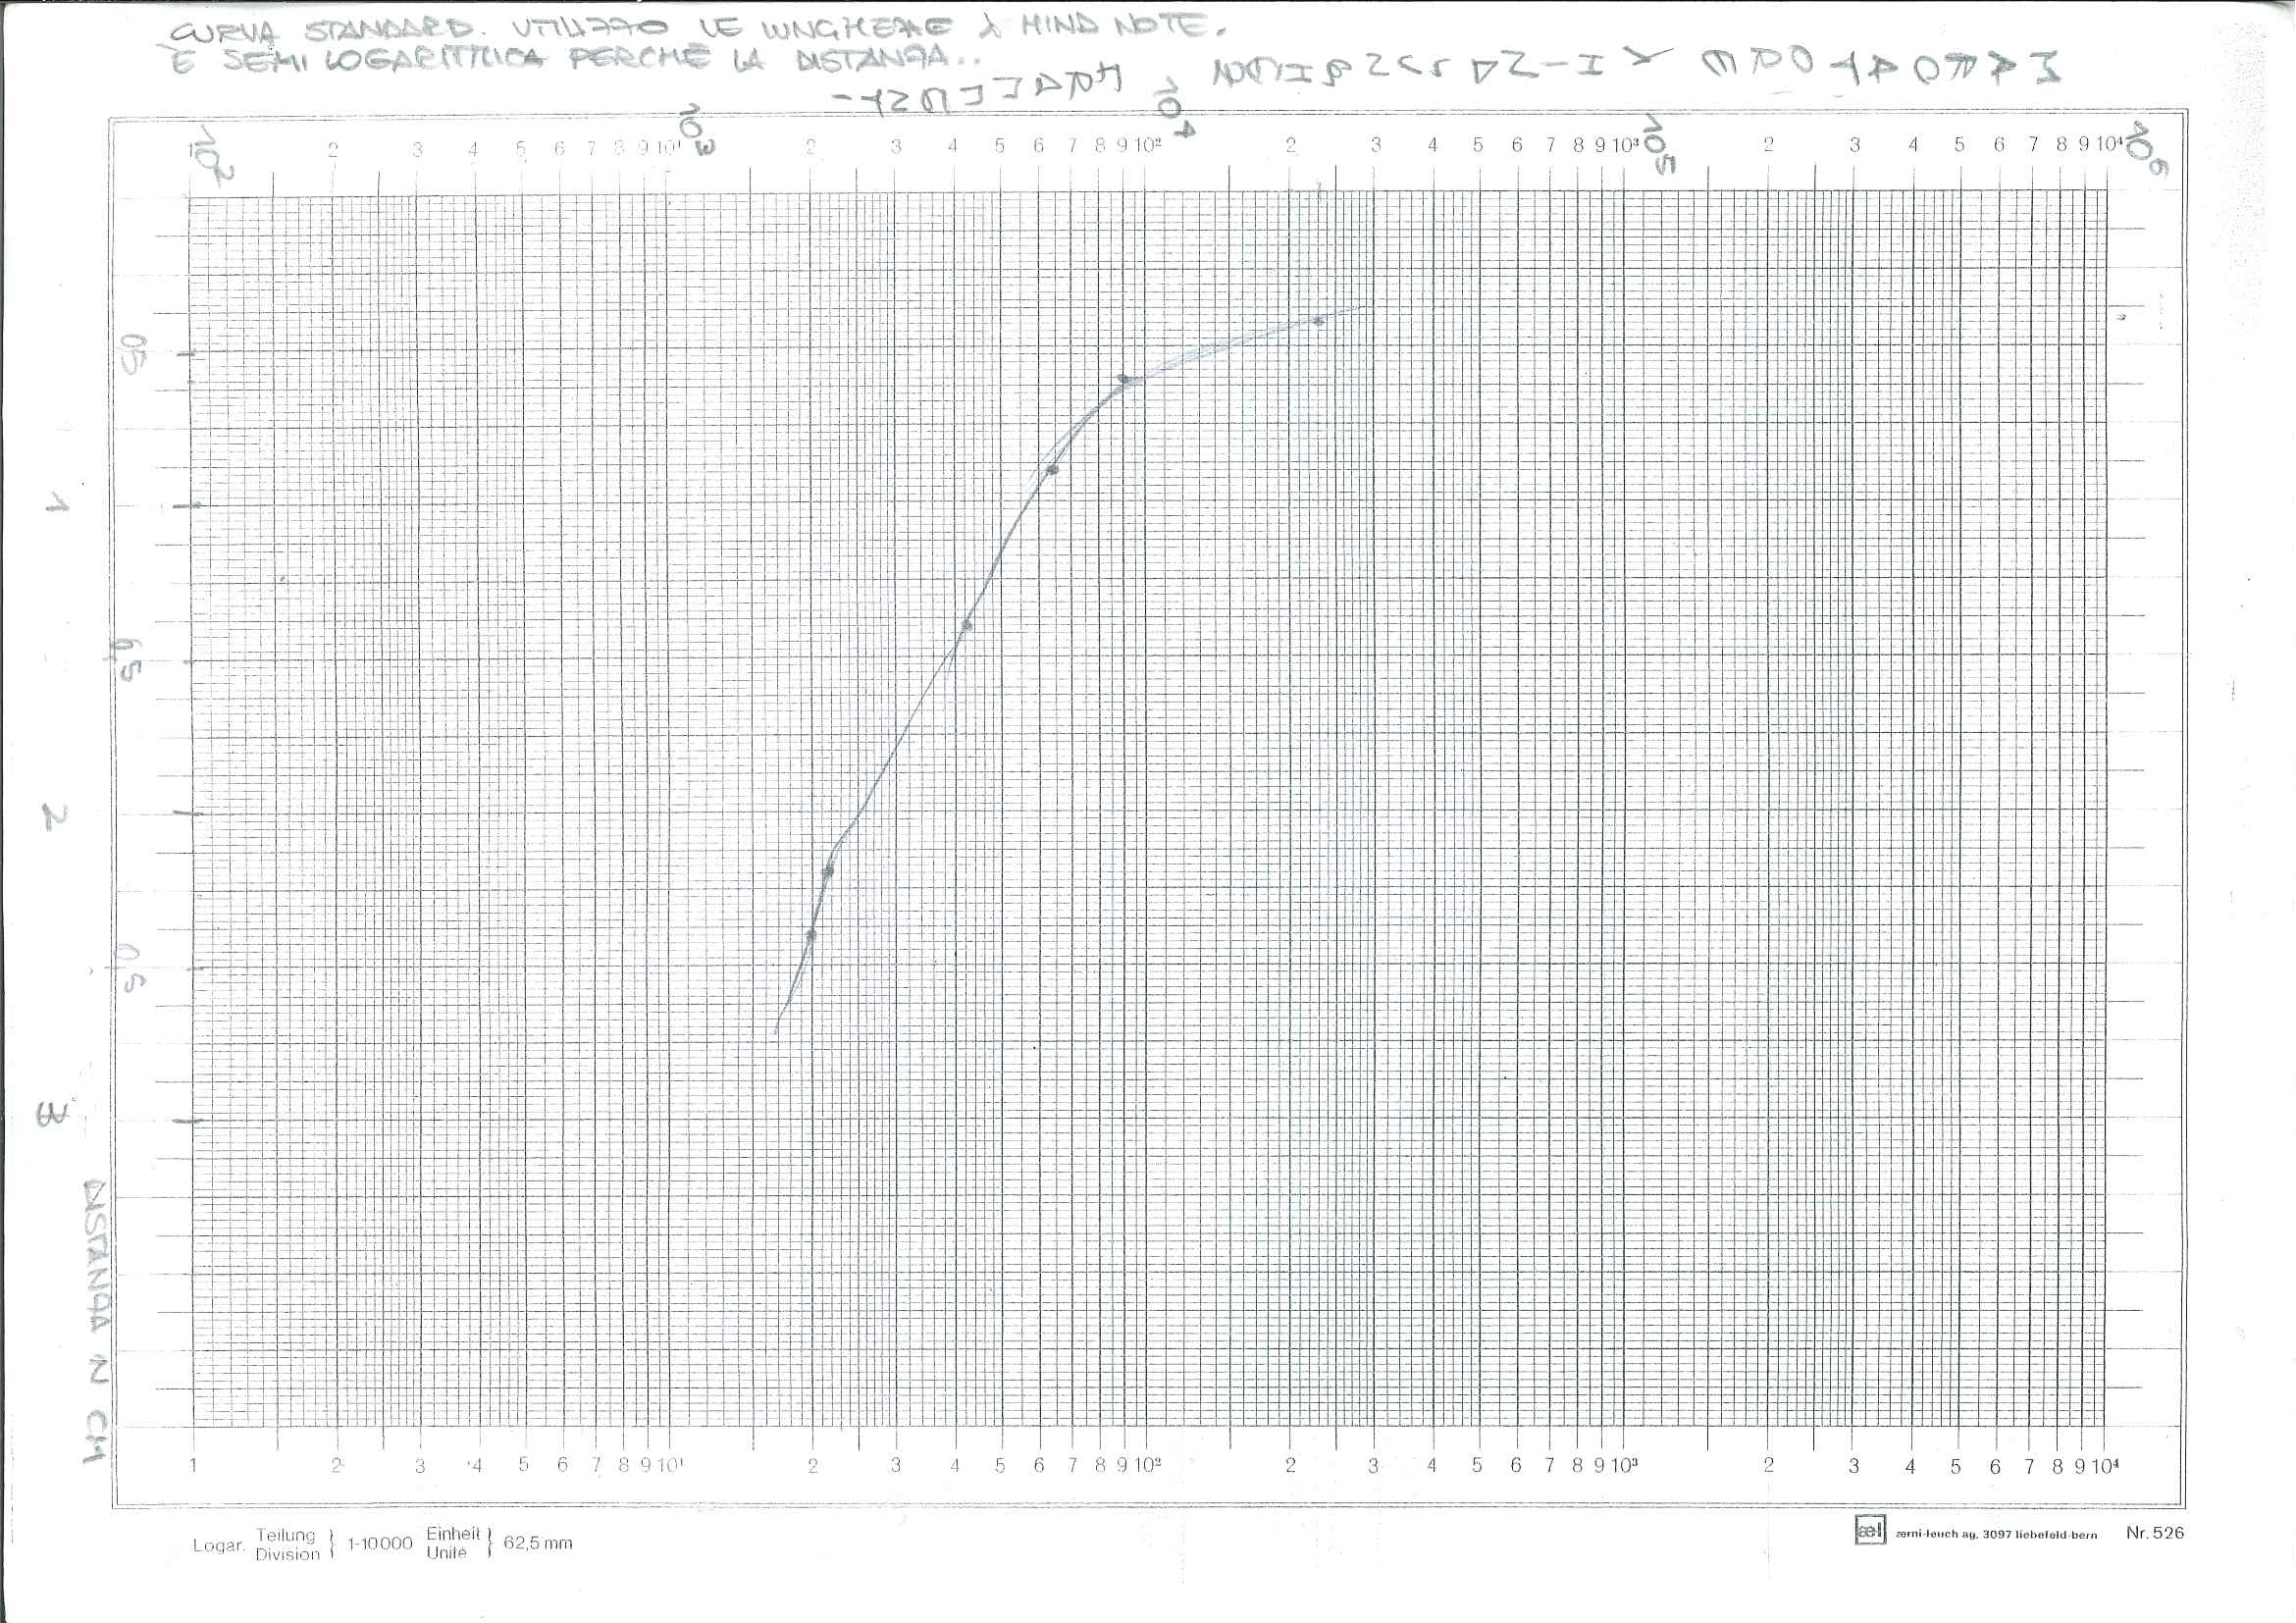
\includegraphics[width=0.8\linewidth]{hind.jpg}
\caption{}
\label{fig:hind}
\end{figure}

\newpage
\header{Laboratorio Metodologie Biomolecolari}{
Corso di Laurea Triennale in Scienze Biologiche \\
Anno Accademico 2017-2018 \\
Modulo: Biochimica -- Professoressa Ilaria Canobbio}

\section{Introduzione -- 12--03--2018}
\subsection{Presentazione teorica del corso}
Nel corso di questo modulo ciò che si vuole ottenere è la purificazione e la caratterizzazione dell'enzima \emph{Piruvato Chinasi I}. La piruvato chinasi I (PKI) è una delle due isoforme\footnote{L'altra isoforma è la Piruvato Chinasi II (PKII).} di questo enzima in E.coli; è composta da una catena di 470 amminoacidi, ha un peso molecolare di circa \SI{50,72}{\kilo\dalton} ed è un omotetramero in cui ciascun monomero è composto da tre domini A--B--C. Questo enzima è caratterizzato da una curva cinetica di tipo sigmoide, tipica degli enzimi allosterici. Gli enzimi allosterici sono regolati da substrati detti modulatori che si legano al sito allosterico presente sull'enzima; se il sito allosterico coincide con il sito catalitico dell'enzima allora avremo un \emph{modulatore omotropico}, ossia il substrato funge da modulatore.Nel caso in cui il sito allosterico è diverso da quello catalitico allora si avrà un \emph{modulatore eterotropico}, che non coincide con il substrato dell'enzima. I modulatori possono essere sia attivatori che inibitori dell'attività enzimatica e, nota importante, il loro legame con l'enzima è reversibile.
La PKI è regolata omotropicamente da \emph{fosfoenolpiruvato (PEP)} ed eterotropicamente da \emph{fruttosio 1,6 bisfosfato}.
La PKI espleta la sua funzione nell'ultima tappa della glicolisi, un importante processo catabolico che porta all'ossidazione parziale di una molecola di glucosio a due molecole di piruvato.
\begin{figure}[htbp]
\centering
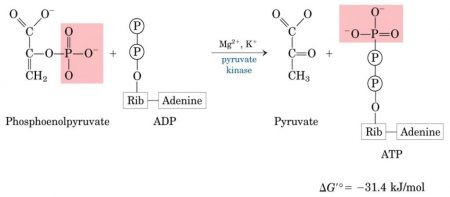
\includegraphics[width=0.8\linewidth]{5.jpg}
\caption{Reazione catalizzata da PK1}
\label{fig:Reazione pk1}
\end{figure}

Per ottenere la PKI purificata, da E.coli, si devono seguire alcuni passaggi che hanno lo scopo di eliminare le altre proteine presenti in cellula, ciò è possibile sfruttando le loro caratteristiche chimico--fisiche.

Per la purificazione, si eseguono le seguenti fasi:

\begin{enumerate}
	\item trattamento al calore
	\item precipitazione con sale
	\item cromatografia a scambio ionico
\end{enumerate}

Per la caratterizzazione, si eseguono le seguenti fasi:

\begin{enumerate}
    \item dosaggio attività enzimatica
	\item dosaggio proteico con metodo Bradford
	\item elettroforesi su gel di poliacrilammide
\end{enumerate}

\section{Purificazione: trattamento al calore e precipitazione con sale -- 13-03-2018}
\subsection{Scopo dell'esperimento}
Il \emph{trattamento al calore} si basa sul concetto che ogni proteina ha una sua temperatura di stabilità. La PKI è termostabile a \SI{50}{\celsius} a differenza dell'altra isoforma PKII, che è termolabile alla stessa temperatura; proprio grazie a questa caratteristica, durante questo passaggio la PKII tenderà a precipitare a differenza della PKI.
Lo scopo di questa fase è quello di denaturare le proteine alterando la loro struttura tridimensionale e causandone la precipitazione in soluzione.

Successivamente viene fatta una \emph{precipitazione con sale}, la cui funzione si basa sul fenomeno \emph{salting in/out}.
Ogni proteina ha un range di solubilità nel quale risulta più solubile (salting in); oltre questo range la proteina tende a precipitare (salting out) perchè gli ioni del sale in soluzione competono con la proteina, legandosi alle molecole d'acqua presenti nello strato di solvatazione attorno alla proteina stessa. Questo provoca l'esposizione di gruppi idrofobici della proteina che interagendo tra loro creando aggregati i quali precipitano.
La PKI ha un range di solubilità compreso tra il 45--65\%,oltre il quale precipita; il sale usato è il solfato d'ammonio \ch{(NH4)SO4} e per stabilire quanti grammi di quest'ultimo si aggiungono in un litro di soluzione, si utilizza la \emph{tabella di Dixon}.

\subsection{Protocollo}
Vengono forniti \SI{5}{\ml} di estratto grezzo\footnote{Dove per estratto grezzo si intende una soluzione contenete tutti i componenti di cellule lisate.} di E.coli. Si prelevano \SI{200}{\ul} e si trasferiscono in una provetta Eppendorf (TC), che si metterà da parte.

Nella provetta rimangono \SI{4,8}{\ml} di estratto grezzo; si esegue dunque il trattamento al calore, in un bagnetto termostatato per 15 minuti a \SI{50}{\celsius}. Attorno alla provetta si mette il parafilm\footnote{Il parafilm è una carta adesiva.} per evitare che entri dell'acqua calda nella provetta.
Dopo aver atteso 15 minuti, si raccolgono tutte le provette e si centrifugano a \SI{4}{\celsius} per 10 minuti a 13000 rpm. Alla fine di ciò tutte le proteine termolabili sono state denaturate e sono precipitate; nella provetta dunque avremo un pellet\footnote{ Il pellet è la fase solida, nella provetta, contenente le proteine precipitate} e un supernatante\footnote{Il supernatante è la fase liquida della provetta.}. Si trasferisce il supernatante in una provetta usando una pipetta Gilson p1000 e poi per misurarne il volume effettivo si sposta in una terza provetta.

Successivamente si procede con il salting out: nella condizione iniziale si ha una concentrazione di sale pari a 0\% di \ch{(NH4)SO4}, aggiungiamo la quantità di sale in grammi riportata sulla tabella di Dixon per giungere ad una concentrazione di 45\%, dunque si impostata la proporzione che rapporta la quantità si sale da aggiungere a microlitri di soluzione e non a litri.
Si aggiunge piano la quantità di sale che risulta dai calcoli facendo attenzione a non versare il sale in un unico gesto perchè altrimenti si sovrasatura la soluzione.
Dopo aver fatto ciò si procede con ulteriore centrifugazione per poi buttare il pellet e conservare il supernatante.
Lo stesso procedimento lo si adopera per passare da una concentrazione di 45\% ad una di 65\%, utilizzando la tabella di Dixon e procedendo con un'ulteriore centrifugazione per poi conservare il pellet.

\subsection{Risultati ed interpretazione}
Alla fine del trattamento al calore si nota che nella provetta il grezzo non ha più lo stesso colore; presenta un colore lattiginoso sinonimo del fatto che alcune proteine, compresa la PKII, sono precipitate.
Anche la precipitazione con sale mostra gli evidenti effetti del salting out, la precipitazione delle proteine che hanno aggregato è visibile nella formazione del pellet.

\section{Purificazione parte 2: cromatografia a scambio ionico -- 15--03--2018}
\subsection{Scopo dell'esperimento}
Per andare avanti nel processo di purificazione della proteina PKI, bisogna ricorrere alla tecnica della \emph{cromatografia}, che sfrutta le caratteristiche chimico--fisiche delle proteine per poterle separare. La cromatografia ha due componenti principiali:
\begin{itemize}
  \item \emph{fase stazionaria}, solida o liquida
  \item \emph{fase mobile}, liquida o solida
\end{itemize}

Esistono diversi tipi di supporti per la cromatografia (su colonna, su sottile strato TLC, su carta) ed esistono diversi tipi di cromatografia (a scambio ionico, gel di filtrazione, di affinità, per interazioni idrofobiche).
Quella adoperata per questo esperimento è la cromatografia a scambio ionico su colonna; questo metodo si basa sulla presenza di gruppi ionizzabili carichi positivamente o negativamente, nelle proteine. La carica netta di queste ultime infatti, dipende dal pH della soluzione e può risultare efficace per la separazione delle proteine.
Un altro dato importante è il \emph{punto isoelettrico} (pI) che equivale al pH quando una molecola ha carica netta pari a zero;
dunque se il pH è \emph{maggiore} del pI, gli amminoacidi hanno carica netta negativa, mentre per pH \emph{minori} del pI, gli amminoacidi hanno carica netta positiva.
La PKI ha un punto isoelettrico pari a 5,65 questo spiega perchè nella tecnica adoperata in questo esperimento si userà come fase stazionaria, uno scambiatore anionico (resina) che possiede gruppi carichi positivamente che attraggono molecole cariche negativamente.

La fase mobile in colonna è un tampone T0 , costituito da Tris, EDTA, 2 mercaptoetano, con un pH di 8,5; questo tampone avendo un pH maggiore del pI conferisce alla PKI una carica netta negativa, in questo modo quest'ultima si lega ai gruppi carichi positivamente della resina. Una volta eliminate tutte le altre proteine presenti nel campione, mediante lavaggi con soluzioni tampone a concentrazioni saline maggiori, stacchiamo la PKI dalla resina modificando le sue interazione ioniche, in questo modo si trasferisce la PKI in provetta.
Per verificare la presenza della PKI, si utilizza lo spettrofotometro, uno strumento che sfrutta la capacità intrinseca degli amminoacidi aromatici come la tirosina e il triptofano, di assorbire la luce a \SI{280}{\nano\metre}. Lo spettrofotometro è dotato di:
\begin{itemize}
  \item \emph{monocromatore} -- che seleziona le lunghezze d'onda impostate
  \item \emph{cuvette in quarzo} -- contiene il campione da analizzare
  \item \emph{rilevatore} -- che trasforma l'intensità dell'onda in un segnale elettrico.
\end{itemize}



\subsection*{Protocollo}
La colonna per la cromatografia a scambio ionico, contiene uno scambiatore anionico, la resina \emph{DEAE sephacel} e viene fornita già preparata.
La colonna è stata lavata con il tampone, dunque si apre la colonna e si fa gocciolare il contenuto lasciandone pochissimo per non lasciarla a secco;infatti una nota fondamentale di tutte le operazioni che si faranno con questo strumento è che la colonna non deve mai rimanere a secco.
Vengono fornite 10 provette Eppendorf e 3 diversi tamponi a base di tampone T0 (Tris, EDTA, 2mercaptoetano), con diversa concentrazione salina di KCl:
\begin{itemize}
  \item Tampone T1 = T0 + \SI{100}{\milli\Molar} di \ch{KCl}
  \item Tampone T2 = T0 + \SI{250}{\milli\Molar} di \ch{KCl}
  \item Tampone T3 = T0 + \SI{1}{\Molar} di \ch{KCl}
\end{itemize}

Per prima cosa si equilibra la colonna, con il tampone T1 poichè questo creerà un giusto ambiente nella colonna.
Dunque si mettono \SI{5}{\ml} di tampone T1 e lo si inserisce in colonna tramite una provetta Pasteur di plastica. Il tampone non si inserisce facendo dei solchi nella resina ma va fatto scendere delicatamente con un movimento circolare altrimenti può alterare il letto della resina.
Nel frattempo si recupera il pellet che si era ottenuto in seguito a precipitazione con sale; si aggiungono \SI{4}{\ml} di tampone T0.
Dei \SI{4}{\ml} presenti in provetta si prelevano \SI{200}{\ul} e si inseriscono in una Eppendorf chiamandola ''PC'', ossia precolonna.
I \SI{3,8}{\ml} rimasti in provetta, si trasferiscono in colonna con una nuova Pasteur; in provetta è presente la PKI e altre proteine che precipiteranno una volta aperta la colonna mentre la PKI rimarrà legata alla resina. Una volta caricato il campione si procede ad un lavaggio della colonna con \SI{10}{\ml} di tampone T1 e poi si procede all'apertura della colonna.
Come già accennato prima, la resina è dotata di cariche positive per cui, quando si inserisce il campione la PKI che è carica negativamente a pH 8,5,si legherà alla resina mentre le proteine cariche positivamente, per repulsione elettrostatica, e quelle neutre tenderanno a cadere in provetta una volta aperta la colonna.
Con il lavaggio fatto, abbiamo staccato dalla resina tutte le proteine presenti nel campione esclusa la PKI; quest'ultima di stacca dalla resina solo alterando le interazioni ioniche, risultato che si ottiene utilizzando un tampone a maggior forza salina.
Dunque aggiungiamo \SI{10}{\ml} di tampone T2 in colonna per poi aprirla e far gocciolare il contenuto in 10 provette Eppendorf, raggiungendo in ciascuna il volume i \SI{1}{\ml}.In queste 10 Eppendorf, se l'esperimento è stato svolto bene, si dovrebbe trovare la PKI.
Per verificare se la PKI è presente, si utilizza uno spettrofotometro che sfrutta la capacità delle proteine, di assorbire la luce;qualora sia presente si rileva un picco.
Si calibra la cuvette di quarzo con tampone T2, per creare il punto zero, dopo di che si rimuove il tampone e si inseriscono i 10 campioni, ottenendo per ciascuno un certo valore.
Tra questi valori ci sarà picco, ossia la provetta in cui è più alta la probabilità di trovare la PKI. \hl{Vedi figura 11}
Si procede costruendo un grafico su carta millimetrata che rappresenta l'andamento dei valori ottenuti dallo spettrofotometro in funzione dei 10 campioni.
L'ultimo passaggio dell'esperimento è costituito dalla rigenerazione della colonna, per eliminare qualsiasi traccia residua di proteine rimaste legate alla resina per via delle loro caratteristiche chimico--fisiche; si aggiungono perciò \SI{10}{\ml} di tampone T3 con la forza ionica maggiore, si apre la colonna e si fa gocciolare in una provetta chiamata \emph{rigenerazione}.

\subsection*{Risultati ed interpretazione}
Il riscontro di questo esperimento si ha principalmente durante l'analisi spettrofotometrica, in quanto i valori ottenuti mostrano chiaramente la presenza di provette in cui l'assorbanza risulta maggiore.

\section*{Caratterizzazione parte 1: dosaggio dell'attività enzimatica -- 21--03--2018}

\subsection*{Scopo dell'esperimento}
Per caratterizzare si userà un saggio dell'attività enzimatica che sfrutta una reazione accoppiata a quella catalizzata dalla PKI. Il fosfoenolpiruvato (PEP), il piruvato, ADP e ATP che sono i reagenti e i prodotti dell'ultima tappa della glicolisi non hanno attività ottica, tuttavia i reagenti della reazione accoppiata, ossia la fermentazione lattica, riducono NADH il quale è otticamente attivo. Il NADH assorbe una lunghezza d'onda di \SI{340}{\nano\metre} e man mano che la reazione accoppiata procede, se la PKI è presente, in provetta si riscontra una diminuzione dei valori di assorbanza per via della diminuzione di NADH.
\begin{figure}[htbp]
\centering
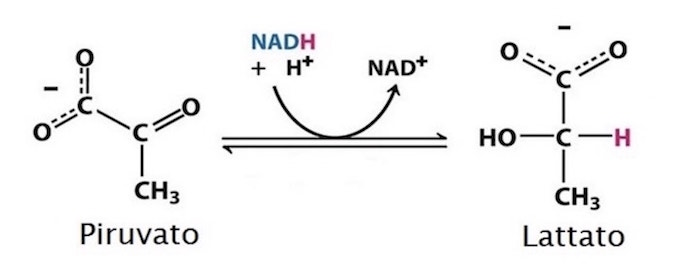
\includegraphics[width=0.8\linewidth]{7.jpg}
\caption{Reazione accoppiata}
\label{fig:reazione accoppiata}
\end{figure}

La reazione viene svolta in condizioni di equimolarità, per cui una mole di PEP viene convertita in una mole di piruvato dall'enzima PKI,a sua volta una mole di piruvato viene convertita nella reazione accoppiata, in una mole di lattato dall'enzima lattato deidrogenasi consumando una mole di NADH.
L’attività enzimatica viene espressa in U/ml, dove
U (unità) è la quantità di enzima che trasforma \SI{1}{\micro\mole} di substrato in un minuto.

\subsection*{Protocollo}
Nella postazione dello spettrofotometro si trovano due provette contenenti:
\begin{itemize}
 \item \emph{MIX} -- contiene tampone Tris (pH 7,5), \ch{MgCl2}, \ch{KCl}, fruttosio 1,6 bisfosfato, ADP, lattato deidrogenasi, NADH.
 \item \emph{Fosfoenolpiruvato (PEP)}
\end{itemize}

Il magnesio e il potassio sono due cofattori, dunque coadiuvano la PKI nella reazione primaria; il fruttosio 1,6 bisfosfato è l'effettore della PKI; l'ADP è l'accettore del gruppo fosfato; la lattato deidrogenasi e il NADH serviranno per la reazione accoppiata.
 Si mettono \SI{360}{\ul} di MIX nella cuvette di quarzo, più \SI{560}{\ul} di PEP e si fa una prima lettura spettrofotometrica che darà un valore iniziale solitamente compreso tra 0,8 0,9. Una volta compiuto questo passaggio si inseriscono in cuvette \SI{20}{\ul} dei campioni che dobbiamo saggiare,uno per volta, precedentemente diluiti ossia:
\begin{itemize}
 \item G -- grezzo, diluito 1:10 (\SI{5}{\ul} di Grezzo, più \SI{45}{\ml} di tampone T0
 \item TC -- trattamento al calore, diluito 1:5 (\SI{10}{\ul} di campione, più \SI{40}{\ul} di tampone T0
 \item PC -- pre colonna, diluito 1:5 (\SI{10}{\ul} di campione, più \SI{40}{\ul} di tampone T0
 \item P -- picco, il campione nel quale abbiamo riscontrato il valore più alto di assorbanza (Eppendorf 6 preparata in seguito a cromatografia), non diluito.
\end{itemize}

 Se la PKI è presente nel campione vedremo una riduzione del valore di assorbanza poichè diminuisce la quantità di NADH, usato nella reazione accoppiata.
Dall'analisi spettrofotometrica di ciascun campione,si ottengono dei grafici (\hl{Vedi figura 12--13--14}) dai quali è possibile ricavare la variazione di assorbanza al minuto. Nel grafico utilizzato per l'esperimento \SI{6}{\cm} corrispondono ad un minuto, perciò per sapere quanti minuti abbiamo in relazione ai centimetri da noi misurati si deve fare una proporzione. Una volta ottenuti i minuti dalla proporzione possiamo calcolare $\sfrac{\Delta A}{\text{min}}$.
Terminato questo passaggio, si moltiplica $\sfrac{\Delta A}{\text{min}}$ per il fattore di diluizione usato per ciascun campione, successivamente si ricava la concentrazione delle specie in soluzione a partire dalla legge di \emph{Lambert--Beer}\footnotemark: $\Delta A= \varepsilon \cdot b \cdot \Delta C$.

\footnotetext{Dove $\varepsilon$ indica il \emph{coefficiente di estinzione molare} che nel caso del NADH è pari a \SI{6222}{\per\mole\per\cm}; $b$ è il cammino ottico e nel nostro caso è pari a \SI{1}{\centi\metre}; $\Delta C$ è la concentrazione espressa in \si{\mole\per\litre}.}
Avendo $\sfrac{\Delta A}{\text{min}}$, conoscendo $\varepsilon$ e $b$ posso calcolare: $$\frac{\Delta C}{\text{min}}=\frac{\frac{\Delta A}{\text{min}}}{\varepsilon\cdot b}$$

Una volta ottenuta la concentrazione espressa in \si{\mole\per\litre},per ogni campione,la si moltiplica per il volume della soluzione nella cuvette, per ottenere le moli effettive: $$\frac{\Delta C}{\text{min}}=\frac{\frac{\Delta A}{\text{min}}}{\varepsilon\cdot b}\cdot \SI{0,9e-3}{\litre}$$

Successivamente, si converte la concentrazione in \si{\mol} così ottenuta in \si{\micro\mole}, moltiplicando per $10^{6}$. Così facendo si ricavano le Unità (U) di attività enzimatica ossia la quantità di enzima che trasforma \SI{1}{\micro\mole} di substrato in \SI{1}{\minute}:

$$U \left(\frac{\si{\micro\mole}}{\text{min}}\right) = \left(
	  \frac{\Delta C}{\text{min}}\si{\mole\per\litre}
      \cdot
      \SI{0,9e-3}{\litre}
    \right)\cdot10^{6}$$

Visto che \emph{l'attività enzimatica} è espressa come \si{\text{U}\per\ml}, come ultimo passaggio occorre fare una proporzione poichè le Unità trovate sono quelle contenute in \SI{20}{\ul} di campione.

\subsection*{Risultati ed interpretazione}
Dai valori ottenuti seguendo i calcoli riportati nel protocollo, io e le mie colleghe di lavoro, abbiamo riscontrato il valore di attività enzimatica più elevato nel campione di Grezzo. Questo perchè abbiamo fatto vari passaggi di purificazione ed è dunque normale che parte della PK1, sia andata persa; infatti il valore più basso l'abbiamo trovato in corrispondenza del picco, ossia il campione ottenuto dopo Cromatografia a scambio ionico e perciò quello che ha subito più passaggi di purificazione. \hl{Vedi tabella 6.}

\section*{Caratterizzazione parte 2: dosaggio proteico tramite metodo Bradford -- 26--03--2018}
\subsection*{Scopo dell'esperimento}
Il dosaggio proteico, a differenza del dosaggio enzimatico, si riferisce alla concentrazione totale delle proteine presenti nel campione e non solo a quella della PK1. La concentrazione proteica è espressa in \si{\milli\gram\per\ml}, alla fine dell'esperimento si deve riscontrare una concentrazione proteica minore ad ogni passaggio di purificazione.
Il metodo Bradford sfrutta le proprietà del colorante \emph{Coomassie brilliant blue}, il legame di quest'ultimo con le proteine determina un assorbimento a \SI{596}{\nano\metre} in soluzioni acide. Ciò che succede è che il colorante forma interazioni non covalenti con amminoacidi basici, ossia carichi positivamente, e aromatici. La quantità di colore che si sprigiona in provetta è direttamente proporzionale alla quantità di proteine presenti nel campione. E' un metodo ad elevata sensibilità quindi misura la quantità di proteine a concentrazioni molto basse.
Visto che si vuole ricavare la concentrazione non nota di una proteina, si sfrutta una curva di taratura con quantità note di un'altra proteina; nel caso di questo esperimento si utilizza la \emph{BSA (albumina serica bovina)}.

L'albumina è una proteina del sangue e trasporta le proteine che vi si trovano e che altrimenti non potrebbero circolare.
Una volta creata la curva di taratura del BSA sarà possibile ricavare la concentrazione proteica presente nei vari campioni espressa in \si{\micro\gram\per\ul}.
Una volta ottenuta la concentrazione, sarà possibile ricavare anche \emph{l'attività enzimatica specifica} espressa in \si{\text U\per\milli\gram}, andando a ragionare sulle unità enzimatiche trovate durante il dosaggio enzimatico.

\subsection*{Protocollo}
La prima operazione consiste nella diluizione dei campioni:
\begin{itemize}
 \item \emph{G} -- diluizione 1:20 (\SI{25}{\ul} di G, più \SI{475}{\ul} di Tampone T0)
 \item \emph{TC} -- diluizione 1:20 (\SI{25}{\ul} di TC, più \SI{475}{\ul} di Tampone T0)
 \item \emph{PC} -- diluizione 1:5 (\SI{100}{\ul} di PC, più \SI{400}{\ul} di tampone T0 )
 \item \emph{P} -- diluizione 1:2 (\SI{250}{\ul} di P, più \SI{250}{\ul} di tampone T0 )
\end{itemize}

Una volta fatte le diluizioni, si preparano 8 provette Eppendorf, contenenti le quantità di reagenti riportati in tabella 2.
\begin{table*}[htbp]
\sffamily\scriptsize
\centering
% \begin{tabular}{r|c|c|c|c|c}
% &&\si{\ug} proteine in cuvette&\si{\ul} BSA standard&\si{\ul} \ch{H2O}&\si{\ul} reattivo\\ \hline
% 1& bianco&0&0&1000&1000\\ \hline
% 2& curva di taratura&2,5&50&950&1000\\ \hline
% 3 &curva di taratura&5&100&900&1000\\ \hline
% 4 &curva di taratura&10&200&800&1000\\ \hline
% &&&&&\\ \hline
% 5 &G diluito&--&50&950&1000\\ \hline
% 6& TC diluito&--&50&950&1000\\ \hline
% 7& PC diluito&--&50&950&1000\\ \hline
% 8& P diluito&--&50&950&1000\\ \hline
% \end{tabular}
\input{table2_new.tab}
\caption{}
\end{table*}

Si procede con analisi spettrofotometrica delle Eppendorf da 1 a 4; si ottengono valori corrispondenti all'Assorbanza ad una lunghezza d'onda pari a \SI{595}{\nm}. Con questi valori e conoscendo le quantità in \si{\ug} di BSA si costruisce una curva di taratura. \hl{Vedi figura 12}
L'equazione della retta è del tipo $y=a+bx$ dove $a$ è pari a zero poichè la retta passa per l'origine e $x$ corrisponde alla concentrazione in \si{\ug},non nota, dei campioni ricavata sulla base dei loro valori di assorbanza (Eppendorf da 5 a 8).
Una volta ottenuti i \si{\ug} per ciascun campione, si moltiplicano questi valori per il fattore di diluizione ottenendo i \si{\ug} totali.
La concentrazione proteica la si ottiene calcolando i \sfrac{\si{\ug}}{\si{\ul}} (=\sfrac{\si{\mg}}{\si{\ml}}) tenendo conto che si hanno \SI{50}{\ul} di campione.
Al termine di queste operazioni si procede a calcolare l'attività specifica\footnote{L'attività specifica (AS) indica quanto enzima PKI è presente nel campione rispetto alle altre proteine.}, la resa\% e il fattore di purificazione tenendo in considerazione tutti i dati raccolti nei precedenti esperimenti.

\subsection*{Risultati ed interpretazione}
Al termine dell'esperimento di purificazione e caratterizzazione ci si aspetta di notare le seguenti variazioni:
\begin{enumerate}
 \item \emph{Attività enzimatica} -- decrescita
 \item \emph{Attività specifica} -- crescita
 \item \emph{Concentrazione proteica} -- decrescita
 \item \emph{Resa \%} -- decrescita
 \item \emph{Fattore di purificazione} -- crescita
\end{enumerate}

Per quanto riguarda i valori 1--3--4, questi sono decrescenti poichè mostrano la perdita delle proteine avvenuta durante le varie fasi della purificazione; mentre la crescita dei valori 2--5, indica quanto è stato corretto il lavoro di purificazione e dunque quanta PKI siamo riusciti ad isolare.
Dai calcoli eseguiti assieme alle mie colleghe di lavoro, ho riscontrato delle anomalie in corrispondenza della concentrazione proteica che risulta essere maggiore nel TC, rispetto a G.
Inoltre anche il valore dell'attività specifica non mostra una crescita netta, influendo dunque sul fattore di purificazione. \hl{Vedi tabella 4 e 5}

\section*{Caratterizzazione parte 3: elettroforesi su gel SDS-PAGE -- 27--03--2018}

\subsection*{Scopo dell'esperimento}
Durante questo esperimento si utilizza la tecnica dell'\emph{elettroforesi su gel SDS--PAGE (PolyAcrylamide Gel Electrophoresis in SDS)}; quest'ultima si basa sul fatto che le molecole dotate di carica si possono muovere con una velocità definita all'interno di un campo elettrico. Questo permette si separare le molecole in base a dimensione e carica. La formula\footnotemark matematica che esprime questo concetto è la seguente:
$\mu=\dfrac{\text{q}\cdot\text{E}}{\text{r}}$.\footnotetext{Dove \begin{itemize}
 \item $\mu$ = mobilità elettroforetica
 \item q =carica (a pH noto)
 \item E = differenza di potenziale applicata
 \item r = raggio della molecola(forma/dimensione)
\end{itemize}}

L'elettroforesi in questione viene svolta su \emph{gel di poliacrilamide}, un gel indicato per la separazione delle proteine.E' composto da una miscela di sostanze tra le quali \emph{acrilamide} e \emph{bisacrilamide} che vengono vendute in stato liquido e in presenza di ammonio persolfato (\ch(NH4)2S2O8) formano legami covalenti tra di loro creando una rete tridimensionale.
Una volta caricato il campione, questo passa attraverso il gel e in base alla dimensione delle maglie del gel le molecole corrono più o meno veloci.
La concentrazione di acrilamide influisce sulla dimensione dei pori del setaccio;nel caso della PKI che pesa \SI{50,72}{\kilo\dalton} si sceglie il gel concentrato al 10\% che serve per separare molecole con dimensioni tra i \SI{21}{\kilo\dalton} e i \SI{100}{\kilo\dalton}.Più bassa è la concentrazione di acrilamide più i pori sono grandi.

Il dissociante per elettroforesi contiene:
\begin{itemize}
 \item SDS \textrightarrow un detergente anionico che denatura le proteine, le carica negativamente e legandosi conferisce un rapporto $\sfrac{\text{massa}}{\text{carica}}$ costante;
 \item Dtt \textrightarrow ossia ditiotreiotolo, un agente riducente che rompe i ponti disolfuro;
 \item Glicerolo \textrightarrow serve a dar peso al campione e a mantenerlo sul fondo del pozzetto;
 \item Blu di bromofenolo \textrightarrow ossia il tracciante, da colore e ci permette di monitorare la corsa elettroforetica.
 \end{itemize}

Il gel si compone di due parti, quella superiore \emph{staking gel}, concentrato al 4\% e con pori più larghi rispetto a quella inferiore \emph{resolving gel}, concentrato al 12\% e con un pH maggiore.
Nella parte superiore, entrano più proteine e vengono impaccate, nella parte inferiore le proteine vengono separate in base al loro PM.

Una volta terminata la corsa elettroforetica il gel viene messo in una soluzione contenete il colorante \emph{blue di Coomassie} che andrà a legare le proteine presenti.

\subsection*{Protocollo}
Si prelevano \SI{50}{\ul} da ciascun campione (G,TC,PC,P) e si trasferiscono in nuove Eppendorf nelle quali verranno aggiunti \SI{25}{\ul} di dissociante.
Una volta preparate queste soluzioni si mettono le provette,esclusa quella contenente G, a riscaldare a \SI{95}{\celsius} per \SI{3}{\text{min}} in uno strumento chiamato \emph{termo mixer}.
Questo passaggio viene fatto per permettere al dissociante di legarsi in maniera ottimale ai campioni, in quanto la temperatura rompe le interazioni molecolari.
Al termine del riscaldamento si andrà ad assemblare la vasca elettroforetica e si caricheranno \SI{20}{\ul} dei campioni tramite una \emph{siringa Hamilton}.
Successivamente si da il via alla corsa fornendo corrente elettrica al sistema; si impostia il voltaggio a \SI{110}{\volt}.
Al termine della corsa si immerge il gel in una soluzione contenente colorante Coomassie e lo si tiene tutta la notte, a seguito della quale verranno fatti passaggi di decolorazione per rimuovere il colore dal gel ma non dalle proteine.



\subsection*{Risultati ed interpretazione}
Al termine del lavoro, si confrontano i pesi molecolari ottenuti con quelli della banda modello. Si può ricavare il PM della proteina di interesse calcolando la distanza percorsa da bande a PM noto.
\begin{figure}[htbp]
\centering
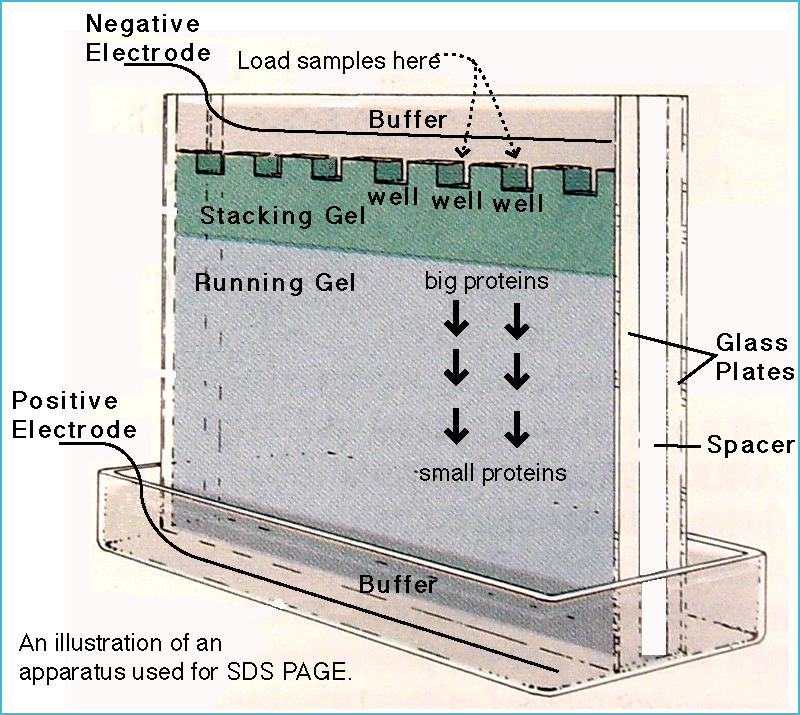
\includegraphics[width=0.8\linewidth]{gel.jpg}
\caption{vasca elettroforetica}
\label{fig:GEL}
\end{figure}

\newpage
\onecolumn{
\section{Allegati modulo biochimica}\label{sec:allegati_modulo2}

\begin{figure}[htbp]
\centering
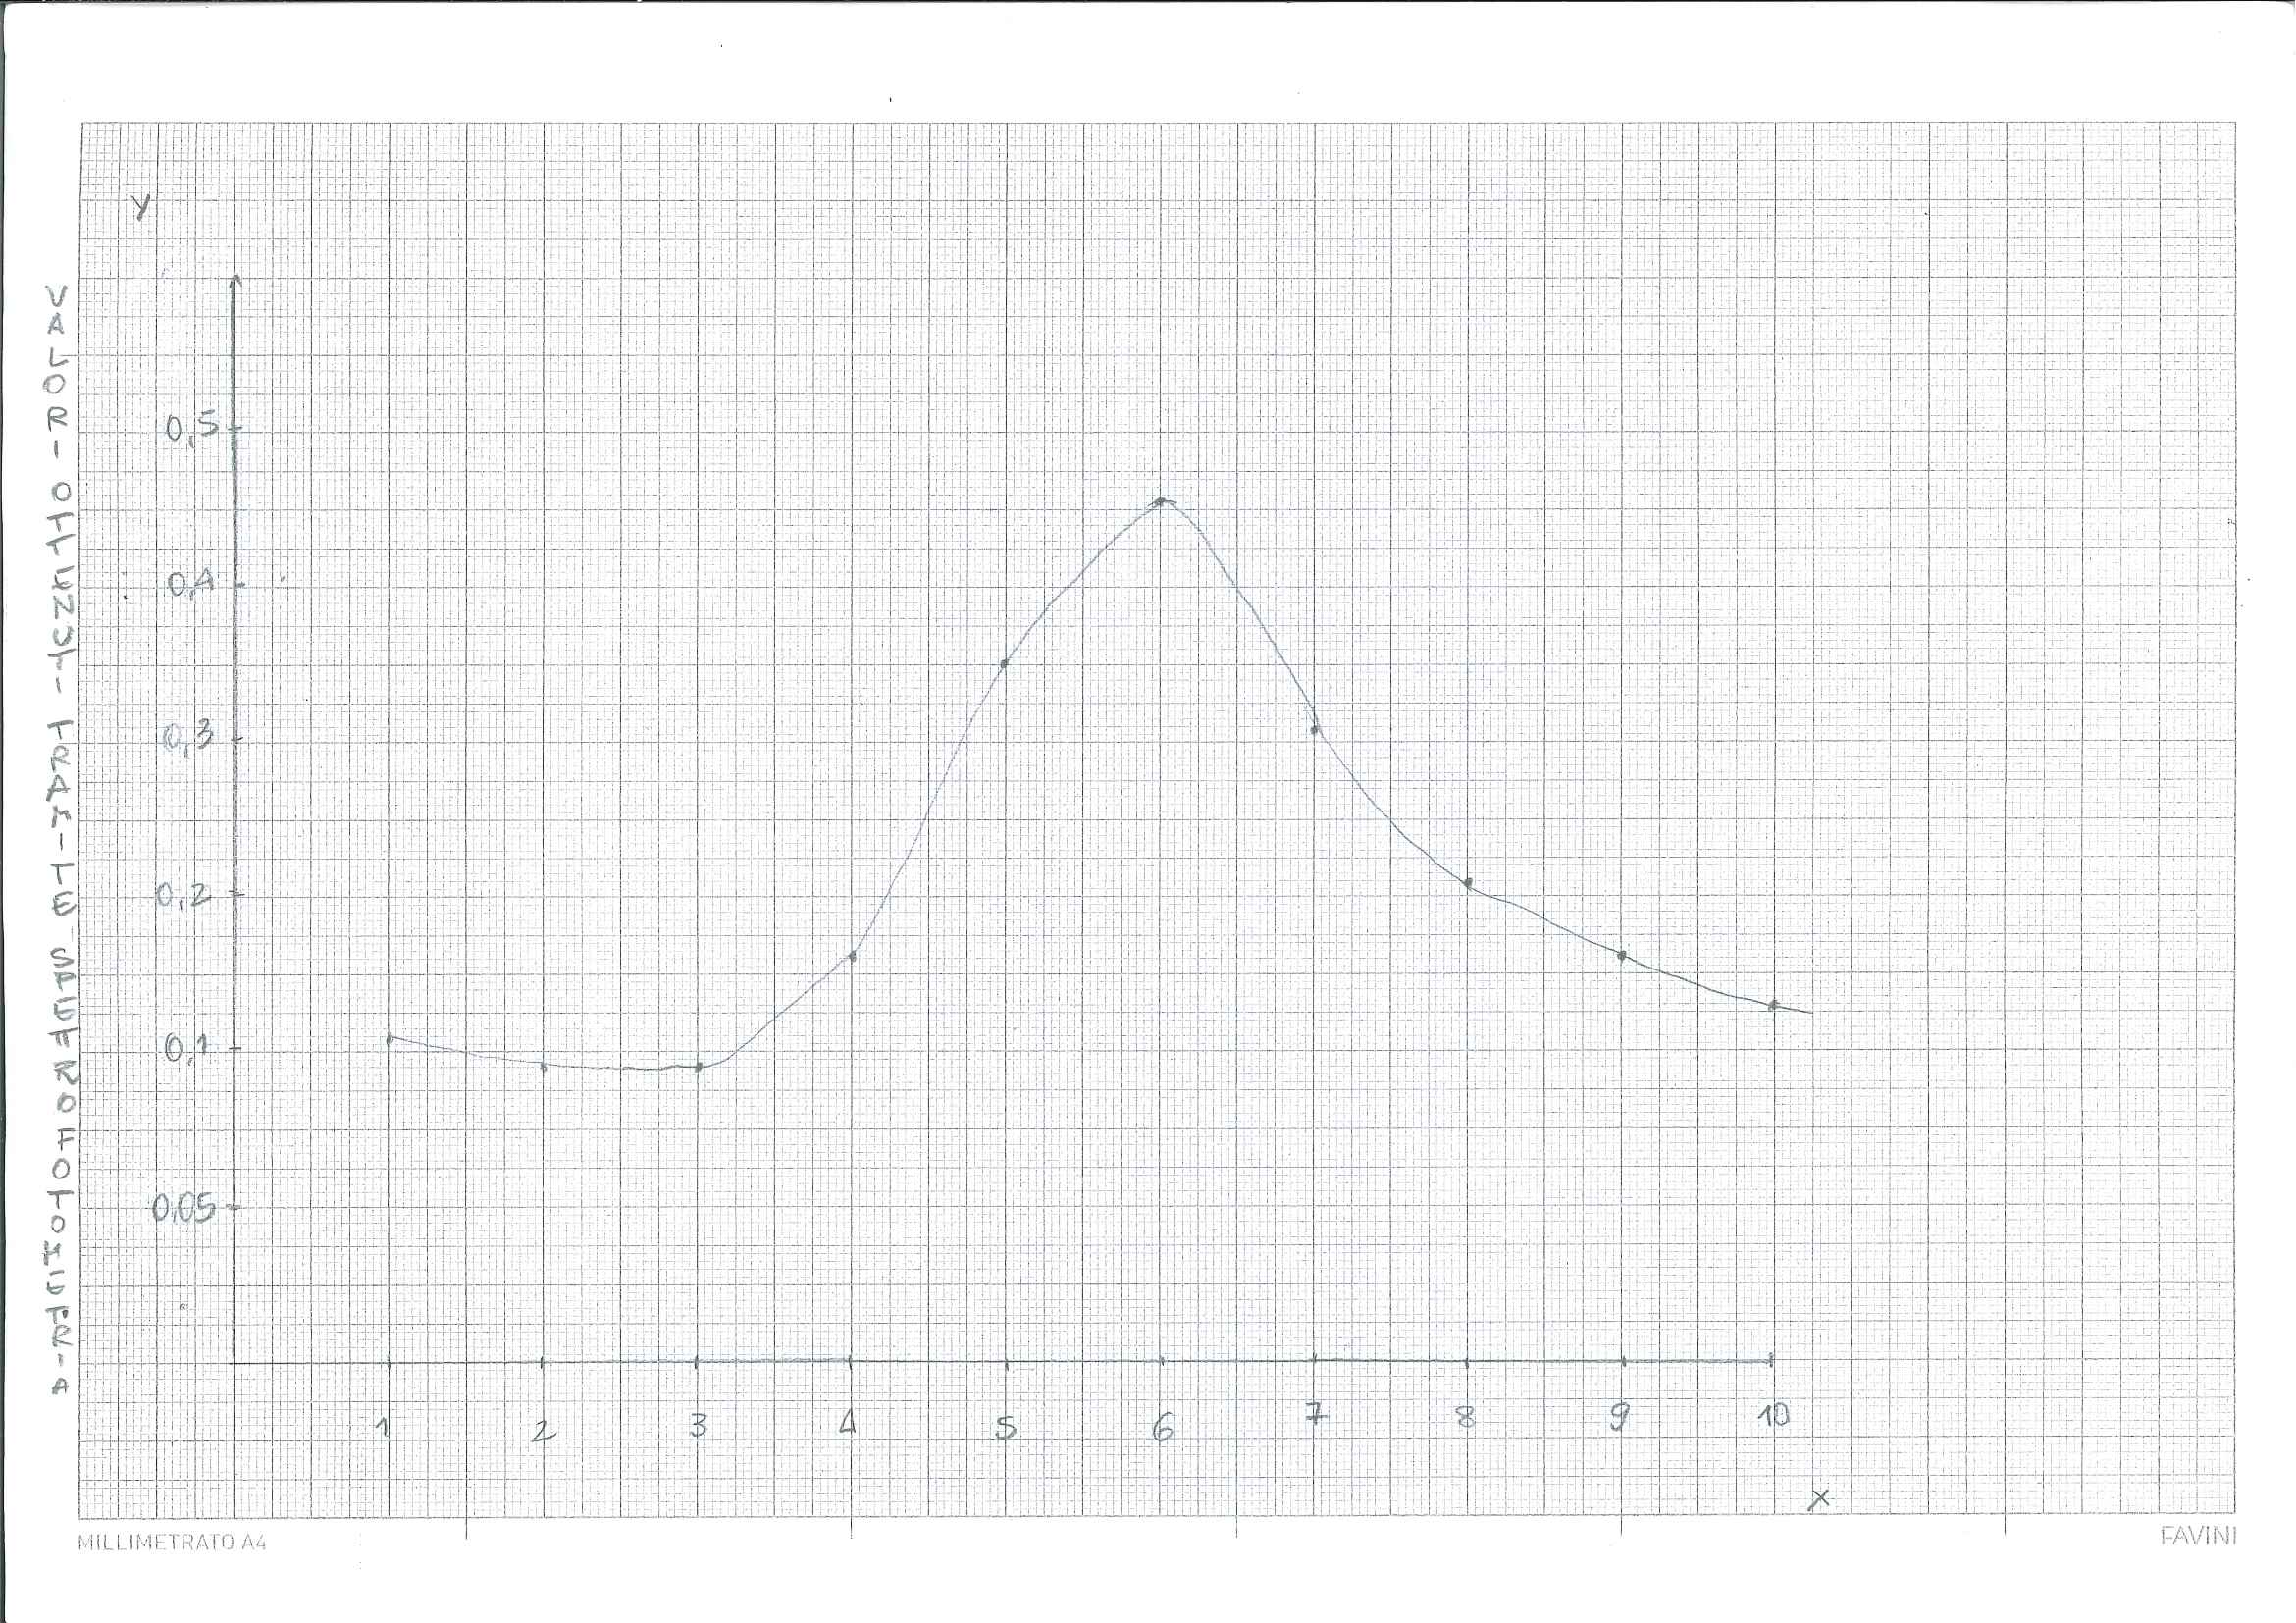
\includegraphics[width=0.8\linewidth]{picco.jpg}
\caption{Grafico che mostra il picco in seguito ad analisi spettrofotometrica dei campioni dopo cromatografia.}
\label{fig:picco}
\end{figure}

\begin{figure}[htp]
\centering
\hfill
\begin{minipage}[b]{.3\columnwidth}
  \centering
  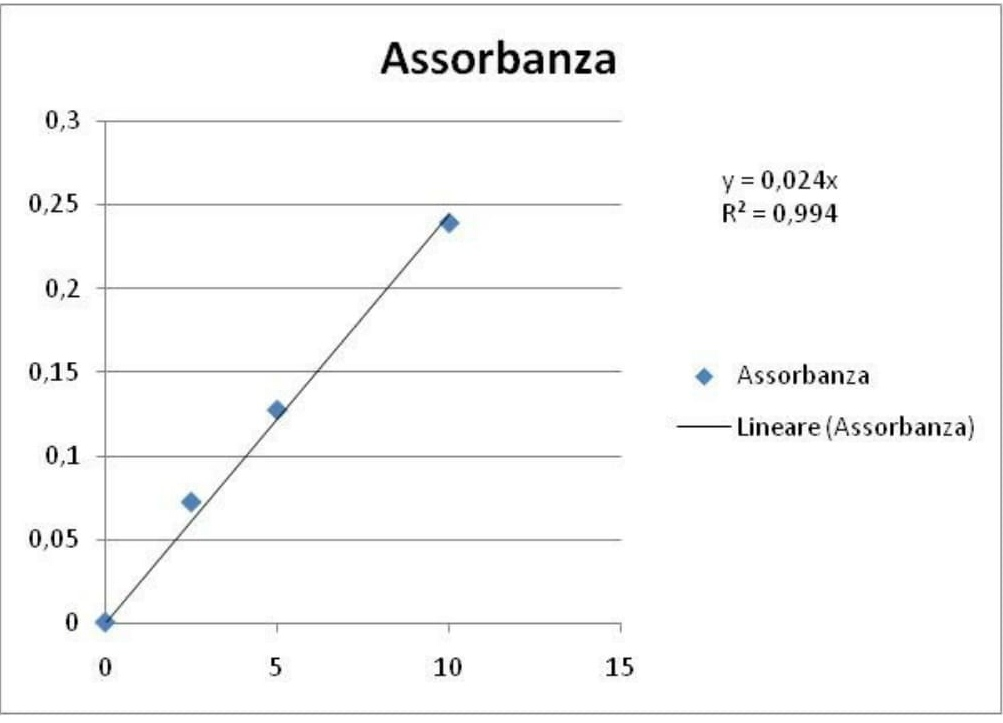
\includegraphics[width=1.5\linewidth]{BSA.jpg}
  \caption{Curva di taratura del BSA con Assorbanza in funzione di \si{\ug}.}\label{fig:BSA}
\end{minipage}\hfill
\begin{minipage}[b]{.3\columnwidth}
  \centering
  \begin{tabular}{|l|l|}
    \hline
    BSA \si{\ug} & Assorbanza \\ \hline
    0        & 0          \\ \hline
    2,5      & 0,072      \\ \hline
    5        & 0,127      \\ \hline
    10       & 0,239      \\ \hline
  \end{tabular}
  \captionof{table}{Dati per la costruzione della curva di taratura in figura 12.}
\end{minipage}\hspace*{\fill}
\end{figure}

\begin{figure}[htbp]
\begin{subfigure}{0.5\linewidth}
\centering
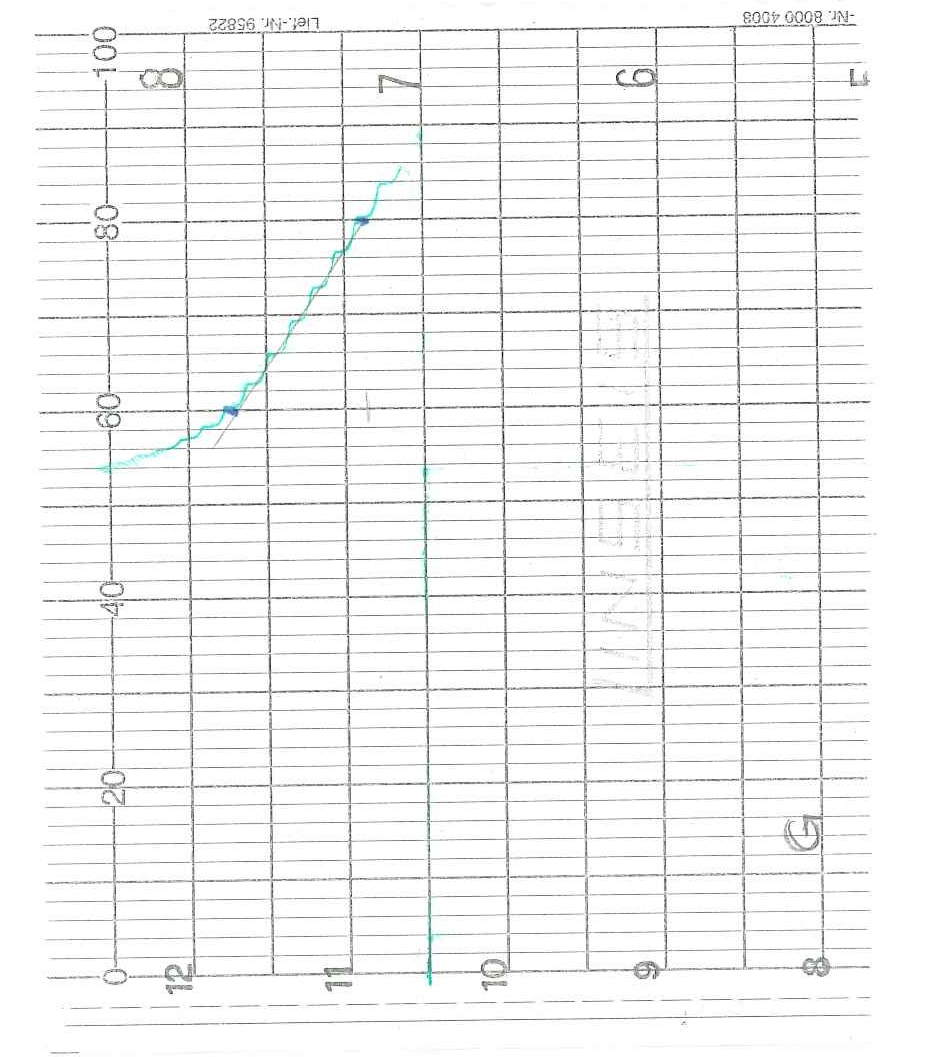
\includegraphics[width=0.8\linewidth]{analisi1.jpg}
\label{fig:analisi1}
\end{subfigure}%
\begin{subfigure}{0.5\linewidth}
\centering
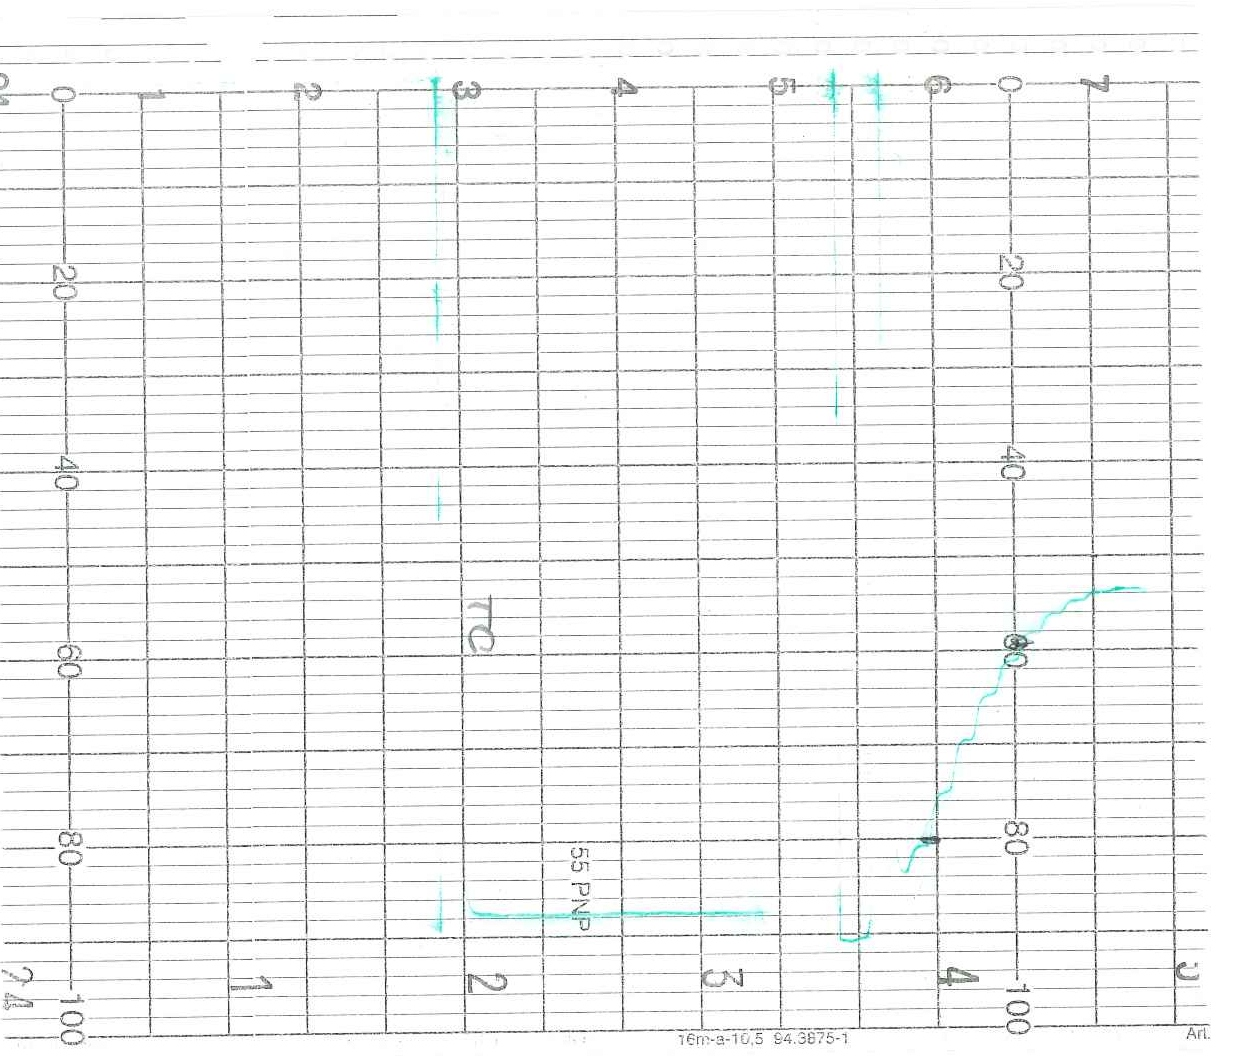
\includegraphics[width=0.8\linewidth]{analisi2.jpg}
\label{fig:analisi2}
\end{subfigure}
\begin{subfigure}{0.5\linewidth}
\centering
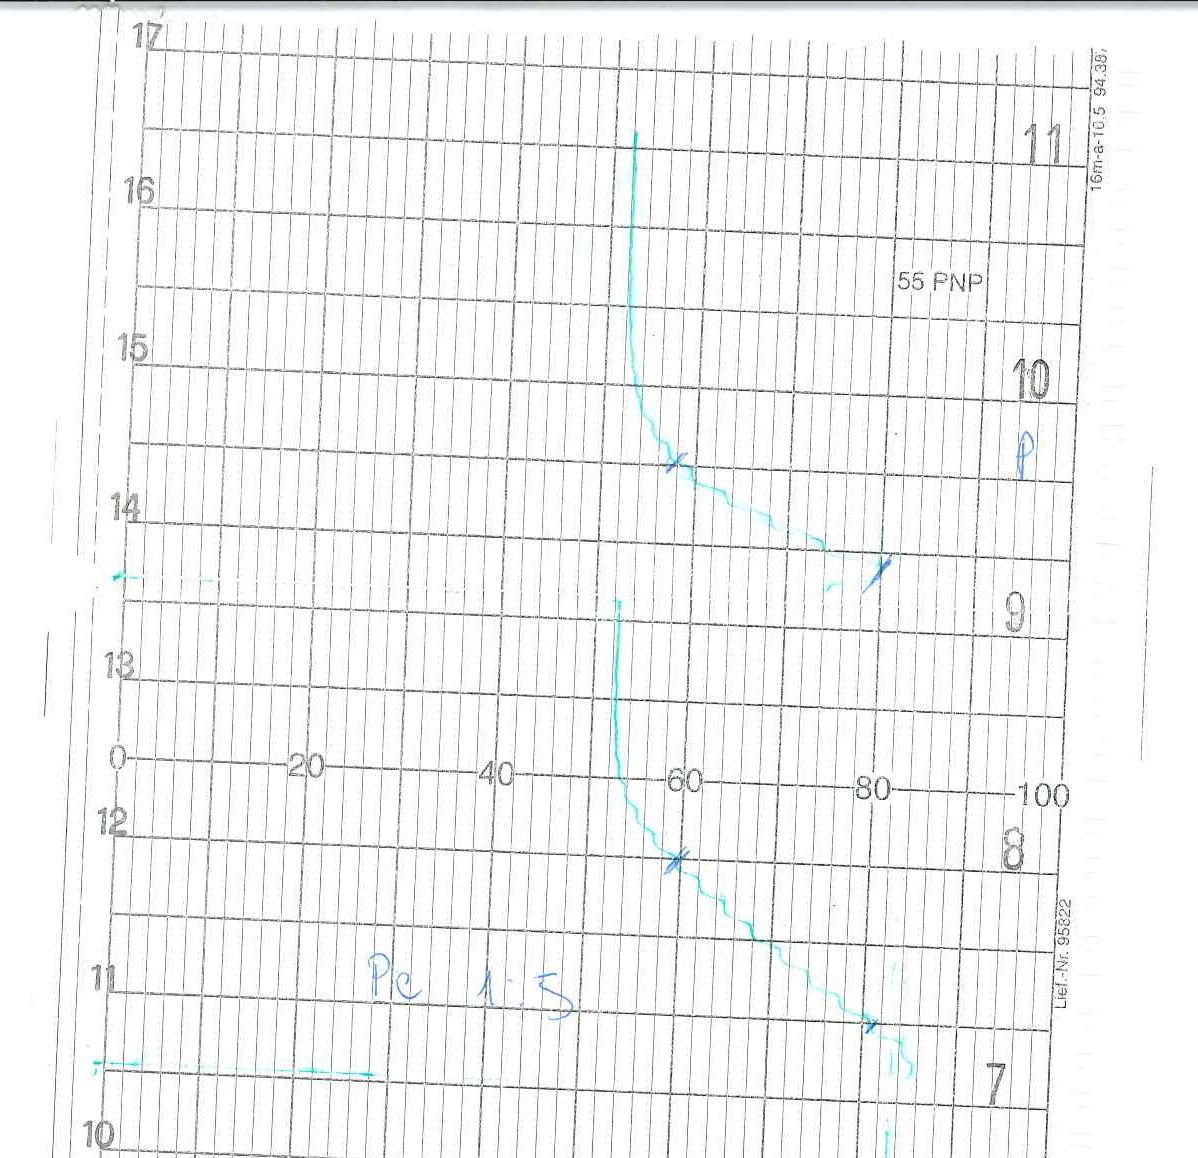
\includegraphics[width=0.8\linewidth]{analisi3.jpg}
\label{fig:analisi3}
\end{subfigure}
\caption{Grafici ottenuti da spettrofotometria per calcolare l'attività enzimatica.}
\label{fig:Risultati}
\end{figure}

\begin{table*}[htbp]
\centering
\begin{tabular}{ccccccc}
\toprule
Campioni & A595 & \si{\ug} cuvette  & diluizione & \si{\ug} totali  & \si{\ug\per\micro\litre} & U/mg (AS)\\
\midrule
G & 0,07 & 2,87 & 20 & 57,4 & 1,148 & 39,13 \\
TC & 0,148 & 6,06 & 20 & 121,2 & 2,424 & 16,52 \\
PC & 0,14 & 5,74 & 5 & 28,7 & 0,574 & 58,77 \\
P & 0,224 & 9,18 & 2 & 18,36 & 0,3672 & 20,67 \\
\bottomrule
\end{tabular}
\caption{}
\end{table*}


\begin{table*}[htbp]
\centering
\begin{tabular}{rlcccc}
\toprule
& U/ml & ml & U tot & Resa\% & Fattore di purificazione\\
\midrule
G & 45,00 & 4,80 & 216,00 & 100,00\% & 1,00 \\
TC & 40,00 & 4,35 & 174,00 & 80,55\% & 0,42 \\
PC & 33,50 & 4,00 & 134,00 & 62,03\% & 1,50 \\
P  & 7,65 & 1,00 & 7,65 & 3,54\% & 0,52 \\
\bottomrule
\end{tabular}
\caption{}
\end{table*}

\begin{table*}[htbp]
\centering
\begin{tabular}{cccccc}
\toprule
Campione & ΔA/min & Δc/min & \si{\umol}/min & U/min  & Fattore diluizione \\
\midrule
G & 0,66 & 1 x 10-4 & 0,9 & 45 & 10 \\
TC & 1,09 & 1,75 x 10-4 & 0,8 & 40 & 5 \\
PC & 0,92 & 1,5 x 10-4 & 0,67 & 33,5 & 5 \\
P & 1,06 & 1,7 x 10-4 & 0,153 & 7,65 & non diluito \\
\bottomrule
\end{tabular}
\caption{}
\end{table*}

}

\header{Laboratorio Metodologie Biomolecolari}{
Corso di Laurea Triennale in Scienze Biologiche \\
Anno Accademico 2017-2018 \\
Modulo: Cristallizzazione -- Professoressa Claudia Binda}

\section*{Cristallizzazione: metodo "Hanging drop" e metodo "Batch" -- 04--04--2018/05--04--2018/06--04--2018}
\subsection*{Scopo dell'esperimento}
L'obiettivo dell'esperimento è la cristallizzazione del lisozima. Il lisozima è un enzima che esplica la sua attività litica sulla parete batterica.

Le proteine sono caratterizzate da una struttura tridimensionale ben precisa definita da : struttura primaria,struttura secondaria, terziaria, quaternaria.
Molti fattori coadiuvano la proteina ad assumere la sua struttura tridimensionale ma il modo in cui dovrà formarsi è contenuto nella sequenza amminoacidica.
Si studia la struttura di una proteina poichè la funzione di una proteina è strettamente correlata alla sua struttura; un'applicazione di questi studi è data dal \emph{drug design} che consiste nella produzione mirata di farmaci. Questi farmaci agiscono legandosi ad un target proteico per esempio un enzima,alterandone l'attività. Bastano poche concentrazioni di questi target proprio perchè hanno un effetto specifico e somigliano ai composti con i quali la proteina interagisce.
Lo studio delle proteine si basa sul fatto che
per vedere un oggetto si usa la luce visibile; si utilizza una radiazione che abbia una lunghezza d'onda con lo stesso ordine di grandezza della distanza tra i punti che voglio risolvere,ossia vedere.
Il problema si pone quando si vogliono vedere le distanze interatomiche in quanto l'ordine di grandezza sta tra i nanometri e gli Ångström, dunque la luce del visibile non basta e si usano i raggi X.
La cristallografia a raggi X consiste nel fatto che un campione, ossia una proteina in forma cristallina, viene colpita da un fascio di raggi X che vengono di conseguenza diffratti. Il cristallo dunque diffrange il fascio in tante direzioni; questi raggi diffratti vengono rilevati tramite detector elettronici e vengono poi elaborati da un computer che crea degli algoritmi matematici che si sostituiscono alle lenti del microscopio. Alla fine si avrà una mappa della densità elettronica che permette di identificare gli atomi in base all'alone di elettroni che c'è intorno a ciascun atomo.

Una molecola cristallizza in modo diverso da come cristallizza un sale; la cristallizzazione è uno step delicato che a volte nelle macromolecole non funziona.
Si sottraggono molecole di acqua dalla soluzione contenente la proteina in modo che le molecole interagiscano tra di loro; infatti se in una soluzione introduciamo sale, ammonio solfato (\ch(NH4)2SO4), questo in acqua dissocia e va ad interagire sia con le molecole d'acqua sia con le proteine in modo da aumentare la solubilità della proteina. Tuttavia se si porta la concentrazione del sale ad un livello molto elevato nell'ordine della molarità succede che il sale compete con le molecole di proteina, sottrae dunque le molecole d'acqua e favorisce le interazioni proteina-proteina.
Le interazioni proteina--proteina portano le molecole a disporsi in modo ordinato, formando dunque un cristallo altrimenti se avviene in modo disordinato si forma un aggregato amorfo.

Relativamente a quanto detto le proteine sono caratterizzate da un \emph{diagramma di fase}, sul quale l'ordinata è la concentrazione della proteina mentre sull'ascissa è riportata la quantità di sale. Per ciascuna proteina possiamo visualizzare la curva di solubilità, al di sotto della quale la proteina è in condizione di \emph{under saturation} ossia il sale ha un effetto solubilizzante.
Al di sopra della curva siamo in \emph{super saturation}, ossia la quantità di sale è tanto alta da far precipitare la proteina, formando un aggregato amorfo.
La zona intermedia \emph{nucleation zone} è caratterizzata da una concentrazione di sale e di proteina che favorisce la formazione dei cristalli di proteina. Si chiama zona di nucleazione perchè si formano dei piccoli nuclei di poche molecole che possono evolvere nella \emph{zona metastabile} nella quale abbiamo un accrescimento dei cristalli.

Si analizzano due tecniche di cristallizzazione:
\begin{itemize}
\item Metodo Batch -- consiste nel mescolare una goccia di soluzione proteica con una goccia di soluzione precipitante (sale o polimero o entrambi);
 la vaschetta verrà ricoperta da olio di paraffina per evitare l'evaporazione.
 \item Metodo Hanging drop -- basato sulla diffusione di vapore, in un microambiente sigillato.
\end{itemize}
\begin{figure}[htbp]
\centering
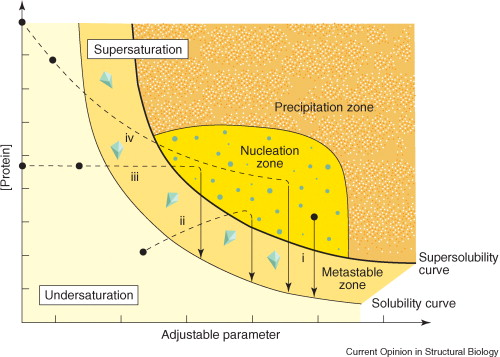
\includegraphics[width=0.8\linewidth]{curva_3.jpg}
\caption{Diagramma di fase}
\label{fig:fig11}
\end{figure}




\subsection*{Protocollo Metodo Batch}
L'agente precipitante è il sale o un'altra molecola che favorisce l'avviamento della cristallizzazione come ad esempio il polimero PEG, ossia polyethylene glycol.
Nell'esperimento si utilizzano entrambi.
Come prima cosa si calcola la quantità di PEG necessaria per ottenere \SI{30}{\ml} di soluzione concentrata al 40\%.
Successivamente si calcola la quantità di \ch{NaCl} da prelevare dallo stock per ottenere \SI{25}{\ml} di soluzione \SI{4}{\Molar}.
Si preparano poi 6 provette Eppendorf contenenti varie quantità di PEG a diverse concentrazioni,\ch{NaCl} (\SI{4}{\Molar}), \ch{CH3COONa} (\SI{1}{\Molar}),\ch{H2O}, per un totale di \SI{1}{\ml} per provetta.
Terminate le preparazioni, si procede a pipettare su piastra per Batch \SI{2}{\ul} di lisozima e \SI{2}{\ul} delle soluzioni precipitanti preparate.
Per sigillare la miscela la piastra è ricoperta da olio di paraffina.
\begin{figure}[htbp]
\centering
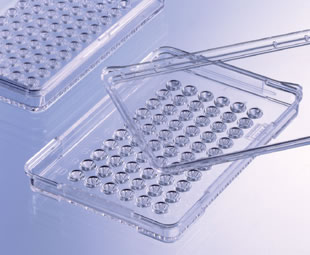
\includegraphics[width=0.8\linewidth]{microbatch.jpg}
\caption{Piastra usata per metodo Bach.}
\label{fig:fig12}
\end{figure}

\subsection*{Protocollo Metodo Hanging drop}
Per questo metodo non si usa il PEG, come agente precipitante ma solo il sale (\ch{NaCl}).
Abbiamo una piccola piastra dotata di 6 pozzetti, disponiamo del grasso attorno a ciascuno di questi in modo da sigillare il vetrino una volta preparato.
Si riempiono i 6 pozzetti con \SI{1}{\ml} delle 6 miscele di cristallizzazione preparate con diverse quantità di \ch{NaCl} a diverse concentrazioni,di \ch{CH3COONa} e \ch{H2O}.
La preparazione dei 6 vetrini avviene pipettando su ciascuno \SI{2}{\ul} di lisozima e \SI{2}{\ul} di soluzione del pozzetto.
Successivamente si ribalta il vetrino con la goccia rivolta verso il basso.
\begin{figure}[ht]
\centering
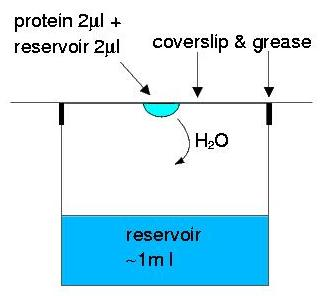
\includegraphics[width=0.8\linewidth]{hanging.jpg}
\caption{Nel metodo Hanging drop, la goccia contenente precipitante e proteina ha una concentrazione minore rispetto alla soluzione precipitante nel pozzetto, dunque a mano a mano che l'acqua evapora, aumenta la concentrazione della goccia e questo porta alla formazione di cristalli.}
\label{fig:fig13}
\end{figure}


\subsection*{Risultati ed interpretazioni}
Si osservano le gocce di cristallizzazione al microscopio. Ci si possono aspettare gocce in cui non è successo nulla; questo perchè le condizioni sono quelle di under saturation quindi la concentrazione di precipitante e proteina non è sufficiente per farle precipitare.
Nel caso in cui si veda una goccia con tanti granulini, probabilmente la proteina è precipitata, quindi si hanno delle concentrazioni elevate di proteine e sale; questo perchè l'evaporazione dell' \ch{H2O} è così alta che le interzioni proteina--proteina avvengono in maniera troppo disordinata, creando un precipitato amorfo. A volte in casi come questo, si notano dei raggi all'interno della goccia poichè i bordi sono disidratati. Ci sono anche situazioni intermedie tra precipitato e cristallo; un precipitato cristallino (crystalline precipitate), non è utile perchè non da una buona diffrazione ma si possono prelevare questi mini cristallini e trasferirli in una nuova goccia,per favorisce la formazione di un cristallo vero e proprio.
Se si ottiene un cristallo perfetto si deve fare un controllo, ossia verificare che non sia stato il sale a cristallizzare.
Possiamo dunque avere vari tipi di precipitati:
\begin{itemize}
 \item Spherulites\textrightarrow possono essere scambiati per mini bolle, sono degli pseudocristalli con disordine interno;
 \item Skin\textrightarrow goccia che appare ricoperta da una specie di membrana, questa non è una condizione ottimale e quando si forma abbiamo una proteina denaturata.
 \item Plates\textrightarrow scagliette attaccate insieme
 \item Needles\textrightarrow aghi
 \item Sea urchin (riccio di mare)\textrightarrow sono tanti piccoli aghetti attaccati insieme.
\end{itemize}

Nel caso del lavoro da me svolto con il metodo Batch, ho evidenziato alcune gocce vuote e alcune gocce in cui erano presenti cristalli; la presenza di cristalli è stata riscontrata a concentrazioni di PEG e \ch{NaCl} crescenti, le gocce vuote sono dovute a un errato pipettamento sulla piastra.
Per quanto riguarda il metodo Hanging drop, ho riscontrato una goccia vuota,corrispondente alla concentrazione più bassa di \ch{NaCl}, tre campioni a concentrazioni di \ch{NaCl} maggiori ( \SI{0,8}{\Molar}-- \SI{1,2}{\Molar}-- \SI{1,6}{\Molar}) in cui ho rilevato la presenza di mini cristallini ed infine due campioni a concentrazioni \SI{2}{\Molar} e \SI{2,4}{\Molar} in cui ho rilevato i ricci.

\newpage
\onecolumn{
\section{Allegati modulo cristallizzazione}\label{sec:allegati_modulo3}
\begin{figure}[htbp]
\centering
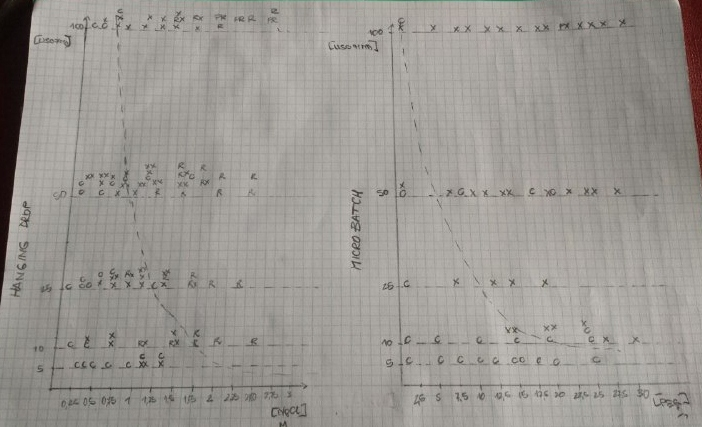
\includegraphics[width=0.8\linewidth]{grafico_binda.jpg}
\caption{Diagramma realizzato in aula raccogliendo i dati di lavoro di tutti gli studenti.}
\label{fig:binda}
\end{figure}


\header{Laboratorio Metodologie Biomolecolari}{
Corso di Laurea Triennale in Scienze Biologiche \\
Anno Accademico 2017-2018 \\
Modulo: Uso Software PyMOL -- Professor Federico Forneris}

\subsection*{Scopo dell'esperimento}
Si utilizza il Software PyMOL, un programma utile alla manipolazione della struttura di una proteina che permette di approcciarsi in modo concreto a tutte le caratteristiche principali della molecola.
Per studiare la struttura tridimensionale di una proteina è necessario poter processare i dati relativi all'analisi cristallografica della stessa. Il cristallo lo si espone ai raggi X, questo perché hanno una lunghezza d’onda vicino all' Ångström (\si{\angstrom}).
Questa unità di misura ci permette di ragionare intorno a valori vicino all’unità, dunque è l’unità di misura più pratica. Quando esponiamo il cristallo ai raggi avviene la diffrazione, questi diffrangono in base alla disposizione delle molecole nel cristallo che sono organizzate in modo ordinato. Quello che si riesce a carpire da uno spettro di diffrazione è la funzione matematica che rappresenta la densità elettronica all’interno del cristallo e da questo si risale alla posizione e al tipo di legami presenti nella molecola.
Ogni punto della struttura tridimensionale che si ottiene è un punto definito dalle coordinate x, y e z che sono caratteristiche per il tipo di interazione chimica presente.
I colori usati in PyMOL, con i quali vengono caratterizzate le molecole sono fissi per gli eteroatomi: azoto blu, ossigeno rosso, fosfato arancione.
Gli idrogeni nelle strutture non sono rappresentati; questo perchè nei legami con gli atomi di idrogeno la densità elettronica si concentra non attorno al nucleo dell’idrogeno ma attorno all’atomo più pesante. L’unico caso in cui si nota qualcosa è quello in cui si ha una risoluzione molto alta e la densità ha una forma a pera che tende in modo minimo anche all’idrogeno. Esistono però tecniche che ci consentono di avere le strutture con idrogeni che non prevedono l'uso di raggi x ma di neutroni.
Nel caso dei neutroni si ha una diffrazione che da una funzione matematica riferita non alla densità elettronica ma alla densità nucleare. Tuttavia per manipolare i neutroni e per attuare questa tecnica si dovrebbe disporre di un reattore nucleare.
In ultima analisi si può dedurre la posizione di un legame idrogeno ragionando sulla presenza di un atomo accettore e un atomo donatore.

\subsection*{Protocollo}
Tra gli esercizi forniti dal Professor Forneris, viene descritto in particolar modo quello riguardante l'emoglobina. Dal pannello menù si apre un file contenente una sessione salvata "1HHO.pdb", appare sulla finestra di PyMOL un dimero cristallografico di emoglobina.
Si procede a generare il dimero complementare tramite il comando "Action"\textrightarrow"generate"\textrightarrow"symmetry mates"\textrightarrow "4A", per poi individuare il dimero corretto ed eliminare tutti gli altri.
Si visualizza la molecola come "Surface" utilizzando il comando "Show"; si creano quattro oggetti separati ossia i monomeri utilizzando il comando "create" in modo che da ciascun dimero si isolino 2 monomeri.
Si utilizza il comando "bg--colorwhite" per poter visualizzare uno sfondo bianco, anzichè nero, per poter osservare al meglio la molecola caratterizzata da quattro colori diversi per ogni subunità.
Per aumentare la qualità della visualizzazione si inserisce un ulteriore comando "util.performance(0)" e si procede a fare un ray--trace dell'immagine visualizzata.
L'emoglobina successivamente viene manipolata in modo da rendere visibili i siti che legano gli atomi di Ossigeno e gli ioni \ch{Fe^2+} del gruppo prostetico eme \hl{(vedi figura 18)}; inoltre si sperimentano i vari modi in cui può essere visualizzata una proteina, come ad esempio cartoon, sticks, spheres.\hl{(vedi figura 19)}

In seconda giornata viene invece analizzata la PK1 scaricando il file dalla Protein data Bank; si visualizza la PK1 e visualizzando la sequenza amminoacidica, sfruttando le coordinate date dal file del Professor Forneris, si riescono ad osservate i domini e le subunità che caratterizzano la molecola.\hl{(vedi figura 20)}

\subsection*{Risultati ed interpretazione}
Le attività svolte durante queste due giornate mi hanno fatto apprendere l'importanza di questo tipo di approccio allo studio della biologia molecolare, che prima non avevo mai valutato. E' stata una piacevole scoperta vedere come l'utilizzo di questo programma sia affascinante in quanto da la possibilità di vedere concretamente ciò che si ottiene in laboratorio. A parer mio è stato come passare dal macroscopico al microscopico, con il pregio di poter vedere dal vivo ciò che teoricamente si può solo immaginare.
E' stata un'esperienza formativa che ha suscitato in me interesse per questo tipo di studio.

\newpage
\onecolumn{
\section{Allegati modulo PyMOL}\label{sec:allegati_modulo4}
\begin{figure}[htbp]
\centering
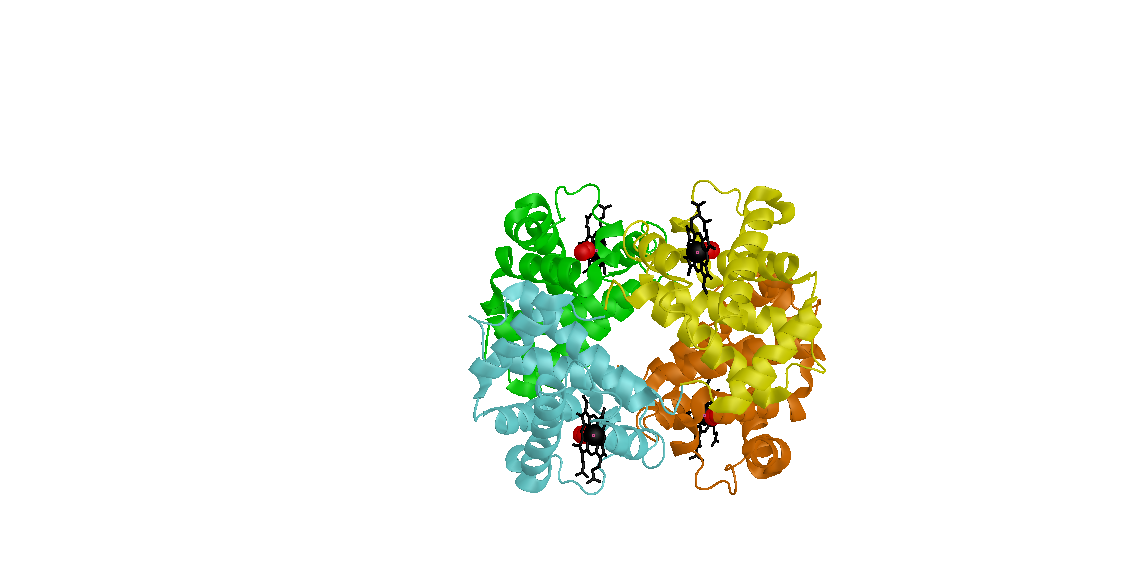
\includegraphics[width=0.8\linewidth]{immagine1.png}
\caption{Emoglobina con ossigeno, ferro e gruppo eme in evidenza.}
\label{fig:emo1}
\end{figure}

\begin{figure}[htbp]
\centering
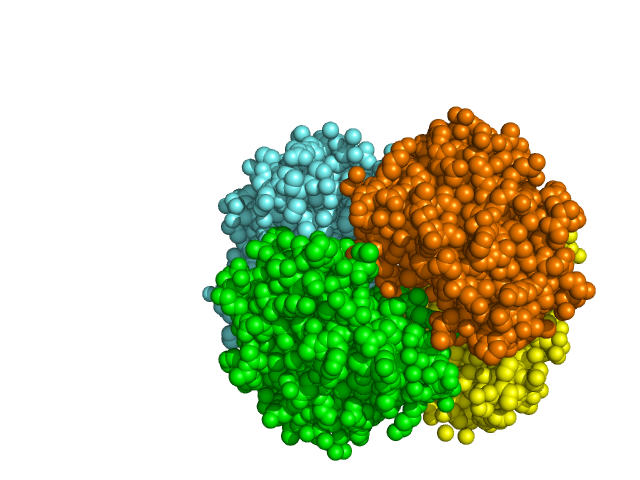
\includegraphics[width=0.8\linewidth]{immagine2.png}
\caption{Emoglobina con rappresentazione a sfere}
\label{fig:emosfere}
\end{figure}

\begin{figure}[htbp]
\centering
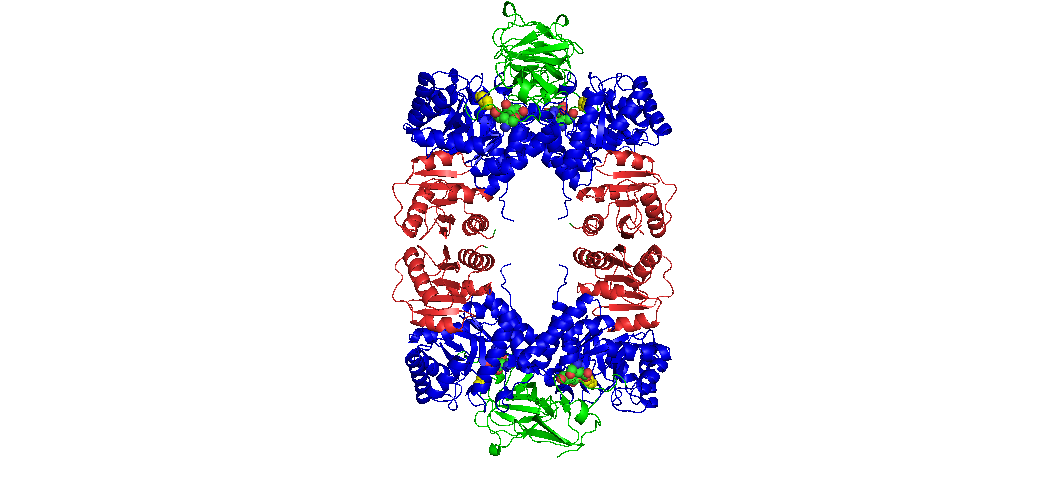
\includegraphics[width=1.0\linewidth]{immagine3.png}
\caption{Struttura tridimensionale PK1}
\label{fig:pK1}
\end{figure}
}



























































\end{document}
